\chapter{Impact des mots-clés en recherche d'information}\label{chap:ri}

Dans le chapitre~\ref{chap:large-scale-eval}, nous avons effectué une évaluation de 9 méthodes de production automatique de mots-clés sur autant de jeux de données dans le but de montrer l'évolution des performances des modèles proposés par la communauté scientifique.
Les méthodes de bout-en-bout ont marqué un tournant dans les performances de la tâche de production automatique de mots-clés avec une amélioration significative dans le cadre d'une évaluation intrinsèque.
Mais, nous avons aussi montré dans le chapitre~\ref{chap:framework} que la majorité des mots-clés de référence auxquels nous avons accès, et donc sur lesquels nous nous évaluons, sont des mots-clés auteurs.
Puis dans le chapitre~\ref{chap:kptimes}, nous avons montré que la qualité de ce type d'annotation rendait difficile l'apprentissage de modèles supervisés et résultait en une évaluation pessimiste. Il est donc important d'envisager d'autres méthodes d'évaluation pour évaluer l'utilité des mots-clés dans une tâche applicative.

Dans ce chapitre, nous allons étudier l'impact de l'enrichissement de l'indexation des documents par des mots-clés dans une tâche spécifique de recherche d'information: la recherche d'articles scientifiques.
Notre objectif est de déterminer si les méthodes de production de mots-clés de l'état de l'art sont suffisamment performantes pour améliorer l'efficacité des systèmes de recherche d'information.
Et dans une plus large mesure si l'enrichissement de documents par des mots-clés améliore l'efficacité des systèmes de recherche d'information.
%Pour cela, nous comparons les résultats obtenus à partir de l'indexation des documents avec et sans enrichissement par mots-clés.
%Plutôt que la classique évaluation intrinsèque vis à vis d'une référence toujours sujette à caution, nous allons étudier la qualité des mots-clés dans une évaluation extrinsèque.
%De nombreuses tâches utilisent des mots-clés, comme la recommandation d'articles~\cite{collins_document_2019} ou les interfaces de navigation~\cite{gutwin_improving_1999} dans les bibliothèques numériques.

%Nous introduisons dans un premier temps les notions nécessaires pour appréhender la problématique de la recherche d'articles scientifiques, ensuite nous décrivons le cadre expérimental dans lequel se situent nos expériences.
Nous décrivons dans un premier temps le cadre expérimental dans lequel se situent nos expériences.
Ensuite, nous présentons nos résultats sur l'enrichissement par des mots-clés en nous intéressant à l'impact des mots-clés produits automatiquement par rapport à ceux de référence.
%
Nous discutons également l'impact des mots-clés présents et absents, et proposons une nouvelle catégorisation des mots-clés absents, plus pertinente dans le cadre de la recherche d'information. 

%Dans un premier temps nous nous intéresserons à l'ensemble des mots-clés, puis aux mots-clés présents et absents.
%L'étude particulière de ces mots-clés nous permettra de discuter la définition actuelle de ces mots-clés présents et absents et de proposer une catégorisation plus fine, plus pertinente dans un cadre de RI.


\section{Cadre expérimental}
\label{sec:ri_framework}

La suite de cette section détaille successivement les collections de test, les systèmes de recherche d'information, les paramètres expérimentaux et les mesures d'évaluation utilisés dans nos expériences.
Nous rappelons tout d'abord les principes généraux de la recherche d'information.

La recherche d'information (RI) est une tâche qui consiste à répondre à un besoin d'information en proposant des documents pertinents.
Les besoins d'information sont exprimés sous forme de requête (un texte décrivant le besoin) qui peut être plus ou moins longue.
Des documents sont rassemblés en collections, dans lesquelles chaque document est indexé -- représenté de manière standardisée -- pour être recherché.
Pour effectuer une recherche, les documents indexés sont ordonnés par un système de recherche d'information par rapport à la requête.


%Les trois grandes étapes du processus de recherche d'informations sont tout d'abord l'indexation des documents, ensuite l'appariement entre une requête et les documents, puis une reformulation du besoin d'information si nécessaire.
%L'indexation se fait majoritairement par sac de mots, l'appariement grâce un schéma de pondération, tel que \tfidf{}, et une distance cosinus entre la requête et les documents.

% Schéma de pondération
%Un moteur de recherche est une interface qui permet de fournir une requête et d'afficher les résultats retournés.
%Les différents moteurs de recherche utilisent chacun des schéma de pondération différents, Google par exemple utilisait l'algorithme PageRank pour privilégier les documents populaires c-à-d. vers lesquels beaucoup de document pointent.



\subsection{Collections de test}

Nous utilisons deux collections de test pour la tâche de recherche d'articles scientifiques.
Ces collections sont composées de notices scientifiques et d'un ensemble de requêtes et jugements de pertinence correspondants.
Les jugements de pertinence indiquent les documents pertinents par rapport à une requête, et donc les documents à retourner en priorité par un système de RI.
La table~\ref{tab:collections} présente les statistiques de ces collections.

\begin{table}[htbp!]
\centering
\resizebox{\textwidth}{!}{
    \begin{tabular}{rcR{6.0}R{3.1}R{3.0}R{2.1}R{2.1}R{2.1}R{2.1}}
    
    %\cmidrule[1pt]{1-9}
    \toprule
            \textbf{Collection} &
            \textbf{Lang.} &
            \textbf{\#Doc.} &
            \textbf{\#Dmots} &
            \textbf{\#Req.} &
            \textbf{\#Rmots} &
            \textbf{\#pert.} &
            \textbf{\#mc} &
            \textbf{\%abs} \\
    \midrule

    NTCIR-2 & en & 322058 & 156.8 &  49 & 11.3 & 28.8 & 4.8 & 38.1 \\
    ACM-CR  & en & 102510 & 158.6 & 169 & 80.0 &  2.9 & 3.1 & 46.4 \\

    %\cmidrule{6-8} %\vspace{-.5em}
    %& & & & \textbf{Avg.} & 603  & 17.3  & 16.8 \\

    \bottomrule

    \end{tabular}
}
\caption{Statistiques des collections de test NTCIR-2 et ACM-CR. La table présente le nombre de documents (\#Doc.) des collections et leur nombre moyens de mots (\#Dmots); le nombre de requête (\#Req.), leur nombre moyen de mots (\#Rmots) et le nombre moyen de document pertinent par requêtes (\#pert.); le nombre moyen de mots-clés (\#mc) par document et le ratio de mots-clés absent (\%abs) par document.}
\label{tab:collections}
\end{table}

% NTCIR-2
\paragraph{NTCIR-2~\cite{kando_overview_2001}}
La collection de test NTCIR-2 a été constituée à l'occasion de la compétition éponyme\footnote{\url{https://research.nii.ac.jp/ntcir/}} pour une tâche de recherche d'articles scientifiques ad-hoc.
Elle contient \num{322 058} notices scientifiques en anglais et 49 requêtes avec jugements de pertinence.
La plupart (\npercent{98,6}) des documents contiennent des mots-clés auteurs (4,8 par document en moyenne).
Les documents couvrent de nombreux domaines, des sciences formelles aux sciences sociales et humaines -- bien que la moitié des documents concernent l'ingénierie et l'informatique.
Les requêtes décrivent des besoins d'informations (un exemple de requête est présenté dans la figure~\ref{fig:ntcir_topic_example}) et sont associées à un ou plusieurs domaines de recherche (le champ \texttt{<FIELD>} des requêtes).
Dans nos expériences, nous utilisons les requêtes courtes (le champ \texttt{<DESCRIPTION>} des requêtes) avec les jugements de pertinence binaires (c'est-à-dire qu'un document est soit \say{pertinent} soit \say{non pertinent}).
Les requêtes comprennent en plus de la description courte et du domaine: un titre court (\texttt{<TITLE>}), une description longue du besoin d'information (\texttt{<NARRATIVE>}) et des mots-clés avec variantes (\texttt{<CONCEPT>}).

%Les expériences de recherche d'articles scientifiques \textit{ad-hoc} sont menées sur la collection de test NTCIR-2~\cite{kando_overview_2001} qui est, à notre connaissance, la seule collection de test disponible pour cette tâche.

\begin{figure}
    \centering
    \begin{minted}[fontsize=\footnotesize,breaklines, breaksymbolleft=]{xml}
<TOPIC q=0145>
<TITLE>Library location</TITLE>
<DESCRIPTION>
  Papers that discuss how the locations of public libraries affect their use
</DESCRIPTION>
<NARRATIVE>
  I want papers that discuss how the locations of public libraries affect the number of visitors, the number of items circulated, the sphere of use, and so on. Both theoretical studies and case studies satisfy this retrieval request. Papers about other types of libraries partially satisfy the request.
</NARRATIVE>
<CONCEPT>
  a. public library, state library, county library, municipal library, 
  b. location characteristics, geographical features, 
  c. numbers of visitors, statistics about visitors, 
  d. volume of circulation, statistics of circulation, 
  e. sphere of use
</CONCEPT>
<FIELD>
  3. Architecture, civil engineering and landscape gardening, 
  8. Cultural and social science
</FIELD>
</TOPIC>
    \end{minted}
    \caption{Exemple de requête extraite du corpus NTCIR-2.}
    \label{fig:ntcir_topic_example}
\end{figure}
% ntc1-e1 187080 docs, 185061 with keywords
% ntc2-e1g 77433 docs, 75081 with keywords
% ntc2-e1k 57545 docs, 57443 with keywords
% all 322,058 documents, 317,585 with keywords (98.6%)

%ACM-CR
\paragraph{ACM-CR~\cite{boudin_acm-cr_2021}}
La collection de test ACM-CR contient \num{102 411} notices scientifiques en anglais et 169 requêtes et jugements de pertinence.
Les documents sont des notices d'articles scientifiques traitant de recherches d'information publiées dans les conférences et revues des groupements d'intérêts spécifiques IR, KDD, CHI, WEB et MOD.
\npercent{69.2} des documents sont annotés en mots-clés auteurs et en contiennent en moyenne 4,5.
Les requêtes sont des paragraphes d'articles scientifiques contenant des citations, ainsi les jugements de pertinence indiquent comme pertinents les articles cités et disponibles dans l'ACM\,DL.
Cette collection permet d'évaluer la tâche de recommandation de citation en contexte, que nous considérons ici comme une tâche de recherche de documents scientifiques avec un besoin d'information exprimé de manière différente -- un exemple de requête est présenté dans la figure~\ref{fig:acmcr_topic_example}.
Par rapport à NTCIR-2 les requêtes sont plus longues 11,3 mots contre 80 pour ACM-CR, et plus bruitées.
En effet, la requête de la figure~\ref{fig:acmcr_topic_example} doit retourner deux articles sur des thématiques différentes: les plongements de mots et l'algorithme TextRank.

\begin{figure}
    \centering
    \begin{minted}[fontsize=\footnotesize,breaklines, breaksymbolleft=]{xml}
<top>
<num> Number: 340120402
<title> Context-Aware Term Weighting For First Stage Passage Retrieval
<desc> Description:
Most first-stage retrieval models such as BM25 and query likelihood use term frequencies (tf) to term importance in a document. A popular alternative to tf are graph-based methods, e.g., TextRank [6]. A few recent work investigated using word embeddings [5] for document term weighting, but most of them only learn a global idf -like term weight because the word embeddings are context-independent. Our work aims to learn tf-like term weights that are context-specific.
<narr> Narrative:
</top>
    \end{minted}
    \caption{Exemple de requête extraite du corpus ACM-CR. Les documents pertinents à cette requête sont les articles référés par \texttt{[5]} et \texttt{[6]}.}
    \label{fig:acmcr_topic_example}
\end{figure}

%Étant donné la taille plutôt limitée de la collection de test NTCIR-2, nous avons mené des expériences supplémentaires sur la recommandation de citations en fonction du contexte~\cite{he_context-aware_2010}, qui consiste à récupérer des citations (documents) pour un texte donné (requête).
%Comme il n'existe pas de collection de test publique dont les documents sont annoté en mots-clés, nous en avons créé une en rassemblant des documents (entrées \hologo{BibTeX}) de la bibliothèque numérique ACM.


\subsection{Systèmes de recherche d'information}

Une fois les documents indexés (représentés sous forme de sac de mots), il est possible de les rechercher, c'est-à-dire de les ordonner selon leur pertinence par rapport à une requête.
Pour calculer la pertinence des documents indexés par rapport à une requête, nous considérons deux systèmes de recherche d'information: Okapi-\bm{}~\cite{robertson_okapi_1999} et Query Likelihood (QL)~\cite{ponte_language_1998}, tous deux implémentés dans l'outil \texttt{anserini}~\cite{yang_anserini_2017}.
Ces deux systèmes adoptent des techniques non supervisées fondées sur des statistiques de corpus pour pondérer les termes. Ils seront donc directement affectés par l'ajout de mots-clés dans un document.

%Nous classons les documents par rapport aux requêtes en utilisant les schémas de pondération standard BM25 et Query Likelihood (implémentés dans la boîte à outils Anserini\footnote{\url{http://anserini.io/}}~\cite{yang_anserini_2017}) sur lesquel nous appliquons la technique d'expansion de requête RM3~\cite{abdul-jaleel_umass_2004} pour obtenir des résultats proches de l'état de l'art~\cite{lin_neural_2019,yang_critically_2019}.


%BM25
\paragraph{Okapi-\bm~\cite{robertson_okapi_1999}}
Le schéma de pondération des termes dans Okapi-\bm{} est calculé par la formule décrite dans l'équation~\ref{eq:bm25_} ci-dessous.\footnote{Par rapport à l'article original: $R = r = 0$ et $k_3 = 0$.}
Similairement à \tfidf{}, \bm{} donne un poids élevé aux mots spécifiques à un document et rééquilibre la fréquence des mots en fonction de la longueur du document.

\begin{align}
\begin{split}
    score(q, d) = & \text{cos}\left(\bm(q), \bm(d)\right) \\
    \bm(d) = & \left[\bm(d, w) | w \in \text{Voc}\right] \\[.5em]
    \bm(d, w) = & \textsc{Tf}_{\bm} *  ln \left(\frac{N - \textsc{Df}(w) + 0.5}{\textsc{Df}(w) + 0.5} + 1 \right) \\[.5em]
    \textsc{Tf}_{\bm} = & \frac{\textsc{Tf}_d(w) * (k_1 + 1)}{\textsc{Tf}_d(w) + k_1 * (1 - b + b * \frac{|d|}{\text{Moy}_{|d|}})}
    \label{eq:bm25_}
\end{split}
\end{align}

Où $\bm(d)$ est un vecteur de taille $|\text{Voc}|$ contenant le poids de chaque mot dans le document $d$, $\bm(d, w)$ le poids du mot $w$ dans le document $d$, $N$ est le nombre de documents dans la collection, $\textsc{Df}(w)$ le nombre de documents dans lesquels le mot $w$ apparaît, $\textsc{Tf}_d(w)$ la fréquence du mot $w$ dans le document $d$, $|d|$ la longueur du document $d$ et $\text{Moy}_{|d|}$ la longueur moyenne des documents de la collection.
%
Les paramètres $b$ et $k_1$ sont des constantes permettant de modifier l'importance de la longueur du document.
%
%L'idée étant qu'un mot ayant une fréquence élevée ou étant spécifique à un document est une indication de son importance. L'intérêt de \bm{} par rapport à \tfidf{} est d'augmenter l'importance d'un mot dans un document si le document est plus court.

%Query Likelihood explications de : https://citeseerx.ist.psu.edu/viewdoc/download?doi=10.1.1.155.1908&rep=rep1&type=pdf et https://www.youtube.com/watch?v=VY3coNGm2Es
\paragraph{Query Likelihood (QL)~\cite{ponte_language_1998}}
QL est un schéma de pondération qui estime le niveau de pertinence d'un document en utilisant la probabilité que la requête ait été générée par le modèle de langage du document. 
Plus formellement, le score de pertinence entre une requête et un document est calculé selon l'équation~\ref{eq:ql}.

\begin{align}
\begin{split}
    score(q, d) = & P(q|d) \\
    P(q|d) = & \prod_{w\in q} P(w|d)^{\textsc{Tf}_q(w)} \\
    P(w|d) = & \frac{\mu}{|d| + \mu} P_{mle}(w|d) + \frac{|d|}{|d| + \mu} P_{mle}(w|C) \\
    %P(w|d) = & \lambda P_{mle}(w|d) + (1 - \lambda) P_{mle}(w|C) \\
    P_{mle}(w|d) = & \frac{\textsc{Tf}_d(w)}{\sum_t \textsc{Tf}_d(t)}
    \label{eq:ql}
\end{split}
\end{align}

Où $P(q|d)$ est la probabilité de générer la requête $q$ à partir du document $d$, $P(w|d)$ la probabilité de générer le mot $w$ à partir du document $d$, $P_{mle}(w|d)$ la probabilité unigramme du mot $w$ dans le document $d$ et $C$ l'ensemble des documents de la collection.

L'usage d'un modèle de langue doit être accompagné d'un mécanisme de lissage.
En effet, si un mot de la requête n'apparaît pas dans le document, $P(w|d)$ sera nul, et $score(q|d)$ aussi.
Ici, nous utilisons le lissage de Dirichlet~\cite{zhai_study_2017} (par défaut dans \texttt{anserini}) qui combine le modèle de langue du document $P_{mle}(w|d)$ et de la collection entière $P_{mle}(w|C)$ pondéré par un paramètre $\mu$ permettant de privilégier le modèle de langue du document plus celui-ci est long.
%L'implémentation d'Anserini utilise le lissage de Dirichlet qui interpole le modèle de langage du document et celui du corpus à en fonction de la longueur du document paramétrée par $\mu$.\footnote{Dans nos expériences $\mu$ est fixé à \num{1000}, selon les paramètres par défaut d'Anserini.}

% Dirichlet smoothing: Jelinek-Mercer (interpolation du LM du doc et du corpus), mais au lieu d'utiliser lambda on utilise une fonction de la longueur du document, (plus un doc est long plus il faut utiliser son LM) $\frac{\mu}{N + \mu} * LM_d + \frac{N}{N + \mu} * LM_c$ et 

% RM3
\paragraph{RM3~\cite{abdul-jaleel_umass_2004}}
Nous utilisons en sus des deux systèmes décrits plus haut une méthode de retour de pertinence simulé, nommée RM3 pour obtenir des résultats proches de l'état de l'art~\cite{lin_neural_2019,yang_critically_2019}.
Le retour de pertinence est une technique permettant à l'utilisateur de préciser sa requête en indiquant les documents les plus pertinents retournés dans une première phase de recherche.
Grâce à ce retour une seconde requête est construite et de nouveaux documents sont retournés.
Le mécanisme de retour de pertinence simulé RM3 automatise ce processus en choisissant les $M$ termes les plus importants parmi les $N$ documents les plus pertinents.
La requête finale est une interpolation de la requête originale et de la nouvelle requête par un paramètre $\lambda$.%\footnote{Dans nos expériences $N$ et $M$ sont tout les deux fixés à 10 et $\lambda$ est fixé à 0,5 selon les paramètres par défaut d'Anserini.}

\begin{table}[!ht]
    \centering
    \begin{tabular}{l|cc}
        \toprule
            \textbf{Système} & 
            \textbf{\map} & 
            \textbf{P@10} \\
            %\textbf{P30}  \\
        \midrule
            
            \textsc{Bm25}+RM3 & \best{35,5} & \best{38,9} \\

            QL+RM3 & 34,4 & 36,1 \\

            1\textsuperscript{er} {\small \cite{fujita_notes_2001}} & 
            31,9 & 37,4 \\
            
            \textsc{Bm25} & 31,9 & 37,1 \\
            
            2\textsuperscript{nd} {\small \cite{murata_crl_2001}} & 
            31,3 & 36,1 \\
            
            QL & 31,2 & 35,1 \\
            
            3\textsuperscript{èm} {\small \cite{chen_berkeley_2001}} &
            26,2 & 33,9 \\
            
        \bottomrule
    \end{tabular}
    \caption{Efficacité de recherche documentaire des systèmes utilisés et des meilleurs systèmes présentés à NTCIR-2.}
    \label{tab:ir_validation}
\end{table}

% title, description,n arrative, and concept
% search for only D

% JSCB3 31.93  based on tf*idf with pseudo-relevance feedback (no info so T+A+K) \cite{fujita2001notes}
% CRL5 31.31 based on BM25 with pseudo-relevance feedback (no info so T + A + K) \cite{murata2001crl}
% Brkly6 26.24 probabilistic model with supervised regression (TITE,ABSE,KYWE, andPJNE) \cite{chen2001berkeley}
% Sstut9 22.67
% Aplee2 19.55
% OASIS5 9.96

%for METH in bm25 bm25+rm3 qld qdl+rm3; do
%    anserini/tools/eval/trec_eval.9.0.4/trec_eval -m map -m p.10 -q \
%        data/ntcir-2/qrels/rel1_ntc2-e2_0101-0149.qrels \
%        data/ntcir-2/output/run.ntcir-2-t+a-all.description.${METH}.txt
%done

% Justification du choix des méthodes
Pour valider le choix des 4 systèmes de recherche choisis pour nos expériences (\bm{}, \bmrm{}, QL et QL+RM3), nous comparons leurs performances avec celles des 3 meilleurs systèmes ayant participé à la compétition NTCIR-2.
Les scores des systèmes sont mesurés à l'aide de la \map{} et de la P@10 (voir chapitre~\ref{chap:framework}).
%La \map{} mesure la qualité globale du classement et la P@10 reflète le nombre de documents pertinents sur la première page des résultats de recherche.
Nous indexons les documents de la même manière que les systèmes participants à NTCIR-2, c'est-à-dire avec le titre, le résumé et les mots-clés auteurs.
Les scores sont présentés dans le tableau~\ref{tab:ir_validation}.
Nous constatons que les systèmes choisis pour nos expériences obtiennent de bons scores, dépassant même le meilleur système participant à NTCIR-2 avec une large avance.
Le 1\textsuperscript{er} système utilise RM3, il n'est donc pas surprenant que \bmrm{} et QL+RM3 soient aussi en tête du classement.
Le 2\textsuperscript{d} système utilise \bm{} ce qui explique la similarité de scores avec le système \bm{}.


%\textcolor{blue}{Experiments in keyphrase generation are conducted on the KP20k dataset~\cite{meng-etal-2017-deep}, which contains 567,830 scientific abstracts with author-assigned keywords (5.4 per doc.~on avg.).
%
%We use that dataset to train and evaluate the outputs of following neural keyphrase generation models: (1)~CopyRNN~\cite{meng-etal-2017-deep} a sequence-to-sequence model with attention, augmented with a copying mechanism~\cite{gu-etal-2016-incorporating}; 
%(2)~CorrRNN~\cite{chen-etal-2018-keyphrase} which extends the aforementioned model with a coverage mechanism~\cite{tu-etal-2016-modeling} to enhance diversity in generated keyphrases; 
%(3)~cat-seq2seq+tg~\cite{chan2019neural} which extends CopyRNN by using the title as an extra input to condition the keyword generation and learns to predict the number of keyphrases to output.}

\subsection{Paramètres expérimentaux}

Deux configurations de base pour l'indexation des documents sont comparées: titre et résumé (\trc{}); et titre, résumé et mots-clés de référence (\trmc{}).
%
Nous ajoutons à ces deux configurations les mots-clés produits automatiquement pour déterminer si ces derniers servent simplement de substituts aux mots-clés de référence ou s'ils les complètent.
%
Nous utilisons toujours les 5 meilleurs mots-clés produits automatiquement pour enrichir l'indexation des documents (sauf si explicitement mentionné).
Ce chiffre correspond au nombre moyen de mots-clés de référence observé sur les collections de test NTCIR-2 et ACM-CR.

Nous utilisons les valeurs par défaut, choisies et justifiées par \texttt{anserini}\footnote{Plus de détail dans le fichier \texttt{SearchArgs.java} du dépôt \href{https://github.com/castorini/anserini/blob/master/src/main/java/io/anserini/search/SearchArgs.java}{\texttt{github.com/castorini/anserini}}}, pour paramétrer nos systèmes de RI.
Pour Okapi-\bm{}, $k_1$ et $b$ sont fixés à 0,9 et 0,4 respectivement.
Avec QL, $\mu$ est fixé à \num{1000} dans le lissage de Dirichlet.
Pour RM3, $M$ et $N$ sont tous les deux fixés à 10 et $\lambda$ est fixé à 0,5.


\subsection{Mesures d'évaluation}

L'ordonnancement des documents par un système de RI est évalué grâce aux jugements de pertinence qui permettent de savoir quels sont les documents pertinents pour une requête.
Avec ces jugements de pertinence, il est possible de calculer des métriques similaires à celles présentées dans le chapitre~\ref{chap:framework}.
Nous rapportons ici la \map{}, calculée sur les \num{1000} premiers documents pour NTCIR-2, et le R@10 pour ACM-CR (tel que recommandé dans \citet{farber_citation_2020} pour la recommandation de citation). Ces métriques sont présentées dans la section~\ref{sub:framework_metrics}.
Nous utilisons aussi le test de Student apparié pour évaluer la significativité statistique de nos résultats au niveau de 0,05~\cite{smucker_comparison_2007}.


\section{Mots-clés de référence et mots-clés prédits}

Dans cette section nous présentons l'impact de l'indexation de mots-clés de référence et de mots-clés prédits sur les scores de recherche d'information.
Tout d'abord nous présentons les résultats généraux, nous investiguons ensuite le nombre de mots-clés à ajouter au document puis l'impact du domaine des documents sur la qualité des mots-clés prédits.


\subsection{Impact des mots-clés sur l'indexation}
\label{sub:ri_impact_pred}

Dans cette expérience, nous indexons les documents de plusieurs manières pour étudier l'impact sur la RI de ces différentes indexations.
Tout d'abord, et comme base de comparaison, nous indexons seulement le titre et le résumé des documents (\tr{}).
Nous indexons ensuite le titre, le résumé et les mots-clés de référence (\trm{}\footnote{Nous utilisons un code couleur pour faciliter l'identification de nos deux configurations de base. Les couleurs ont été choisies de manière arbitraire.}).
\`A ces deux indexations, nous ajoutons des mots-clés prédits par la méthode à base de graphe MPRank, la méthode supervisée Kea\footnote{Entraînée sur l'ensemble de validation de KP20k.} et les méthodes neuronales CopyRNN et CorrRNN (décrites plus en détails dans les chapitres~\ref{chap:introduction} et \ref{chap:framework}).

% Lecture du tableau
Les scores des systèmes de recherche d'information qui indexent les documents et différents mots-clés sont reportés dans le tableau~\ref{tab:ir_results}.
Les colonnes du tableau présentent les scores de \map{} obtenus avec les systèmes \bm{} et QL avec et sans retour de pertinence simulé RM3.
Nous obtenons des scores de \map{} entre 29,5 et 32,9 pour l'indexation \tr{} et entre 31,2 et 35,5 pour l'indexation \trm{}.
Quel que soit le système d'indexation, nous constatons que l'ajout des mots-clés de référence apporte une amélioration des scores par rapport à une indexation ne les exploitant pas.
Lorsque nous ajoutons des mots-clés prédits automatiquement, nous obtenons des scores de \map{} entre 29,7 et 35,0 pour l'indexation \tr{} et entre 31,6 et 37,1 pour l'indexation \trm{}, soit une augmentation moyenne de $+$0,8 et $+$0,5 par rapport aux configurations sans mots-clés prédits.
Notons que l'ajout de mots-clés prédits augmente moins les scores dans la configuration \trm{} que la configuration \tr{}, 1,0 et 0,6 pour CopyRNN par exemple.
Ceci est dû au fait que certains mots-clés prédits sont redondant avec ceux des auteurs. En effet, les méthodes de production de mots-clés sont conçues pour répliquer l'annotation de référence.
Ces résultats montrent qu'avec un système donné, l'ajout de mots-clés prédits augmente les scores de \map{} pour la majorité des configurations par rapport à nos deux configurations de base sans et avec mots-clés de référence.

% Commentaire baisse de score
Nous constatons un cas où le score baisse avec la méthode CorrRNN et le système QL+RM3 pour l'indexation \trm{}. 
%Nous remarquons aussi quatre cas où il n'y à pas d'amélioration, avec les systèmes \bm{} et \bmrm{} et la méthode MPRank pour les deux configurations, et \bm{} et CorrRNN pour \trm{}. 
La baisse de score de \map{} de 0,1 peut être due au mécanisme de retour de pertinence simulé qui peut faire \say{dériver sémantiquement} la requête originale par les termes qui lui sont ajoutés. Nous étudions ce cas plus en détail dans la section~\ref{sec:derive_semantique}.

\begin{table}[!ht]
    \centering
    \setlength{\tabcolsep}{4pt}
    \resizebox{.7\textwidth}{!}{%
\begin{tabular}{l|c@{\hspace*{0mm}}r c@{\hspace*{0mm}}r c@{\hspace*{0mm}}r c@{\hspace*{0mm}}r||c@{\hspace*{0mm}}r}
    \toprule
    \textbf{Indexation} & \multicolumn{2}{c}{\textbf{BM25}} & \multicolumn{2}{c}{\textbf{+RM3}} & \multicolumn{2}{c}{\textbf{QL}} & \multicolumn{2}{c||}{\textbf{+RM3}} & \multicolumn{2}{c}{Moy.} \\

    \midrule
    \tr      & \multicolumn{2}{c}{29,6} & \multicolumn{2}{c}{32,8} & \multicolumn{2}{c}{29,5} & \multicolumn{2}{c||}{32,9} & \multicolumn{2}{c}{31,2} \\
    + MPRank      & 29,7 & \ddiff{0,1} & 33,0 & \ddiff{0,2} & 29,8 & \ddiff{0,4} & 33,0 & \ddiff{0,1} & 31,4 & \phantom{0}\ddiff{0,2} \\
    + Kea (KP20k) & 30,3 & \ddiff{0,7} & 33,9 & \ddiff{1,1} & 30,3 & \ddiff{0,9} & 33,5 & \ddiff{0,6} & 32,0 & \ddiff{0,8} \\
    + CorrRNN     & \sign{31,6} & \ddiff{2,1} & \bests{35,0} & \ddiff{2,2} & \sign{30,9} & \ddiff{1,4} & 34,1 & \ddiff{1,2} & 32,9 & \ddiff{1,7} \\
    + CopyRNN     & \sign{31,4} & \ddiff{1,9} & \sign{34,8} & \ddiff{2,0} & \sign{31,2} & \ddiff{1,7} & 33,9 & \ddiff{1,0} & 32,8 & \ddiff{1,6} \\
    
    \midrule
    \trm       & \multicolumn{2}{c}{31,9} & \multicolumn{2}{c}{35,5} & \multicolumn{2}{c}{31,2} & \multicolumn{2}{c||}{34,4} & \multicolumn{2}{c}{33,2} \\
    + MPRank      & 32,0 & \ddiff{0,1} & 35,8 & \ddiff{0,3} & 31,6 & \ddiff{0,4} & 34,7 & \ddiff{0,3} & 33,5 & \ddiff{0,3} \\
    + Kea (KP20k) & 32,1 & \ddiff{0,2} & 36,0 & \ddiff{0,5} & 31,8 & \ddiff{0,6} & 34,7 & \ddiff{0,3} & 33,6 & \ddiff{0,4} \\
    + CorrRNN     & 32,4 & \ddiff{0,5} & \sign{36,9} & \ddiff{1,4} & 32,0 & \ddiff{0,8} & 34,3 & \ddiff{-0,1} & 33,9 & \ddiff{0,7} \\
    + CopyRNN     & 32,5 & \ddiff{0,5} & \bests{37,1} & \ddiff{1,6} & 32,2 & \ddiff{1,1} & \sign{36,0} & \ddiff{1,6} & 34,4 & \ddiff{1,2} \\

    \bottomrule
    \end{tabular}

    }
    \caption{Scores de \map{} sur la collection NTCIR-2 pour les systèmes de recherche documentaire utilisant différentes configuration d'indexation. La différence de score avec la configuration sans mot-clés prédits est affiché en gris.
    Les symboles \da{} et \dda{} indiquent la significativité par rapport à \tr{} et \trm{} respectivement.}
    \label{tab:ir_results}
\end{table}

% Commentaire des résultats
%
% Les scores augmentent plus on rajoute de mots-clés, donc auto et auteurs sont complémentaire.
Plus généralement, les améliorations de l'efficacité de recherche sont significatives lorsque les documents sont enrichis par l'union des mots-clés prédits et des mots-clés de référence, ce qui indique que ces deux types de mots-clés se complètent.
Cela suggère aussi que les mots-clés prédits sont toujours utiles pour la recherche de documents scientifiques et qu'ils gagneraient à être utilisés même lorsque des mots-clés de référence sont fournis.


Les résultats obtenus avec CopyRNN sur cette évaluation extrinsèque contredisent ceux obtenus lors de notre évaluation intrinsèque (dans le chapitre~\ref{chap:large-scale-eval}) qui montrait la supériorité de CopyRNN par rapport aux autres méthodes de génération de mots-clés.
Ici, CopyRNN et CorrRNN obtiennent des scores similaires: pour une indexation \tr{} CopyRNN et CorrRNN obtiennent des scores de \map{} de 32,1 et 32,0 en moyenne; pour une indexation \trm{} CopyRNN et CorrRNN obtiennent en moyenne 33,8 et 33,7.
Nous comparons ces résultats à l'évaluation intrinsèque de la production de mots-clés sur NTCIR-2 (dans le tableau~\ref{tab:kg_intrinsic}) dans laquelle CopyRNN obtient une F@5 de 23,9 et CorrRNN de 22,3.
Les performances de production de mots-clés de CopyRNN sont supérieures mais l'impact sur la recherche d'information est similaire.
Ces constats encouragent l'utilisation de cette tâche de recherche d'information pour évaluer de manière extrinsèque la production automatique de mots-clés.

\begin{table}[ht!]
    \centering
    %\resizebox{.48\textwidth}{!}{%
    \begin{tabular}{l|cccc}
        \toprule
            \textbf{Méthode} & 
            \textbf{~KP20k~} & \textbf{NTCIR-2} &
            \textbf{KPTimes} & \textbf{ACM-CR} \\
        \midrule
        % Scores sans heuristiques
        MPRank  & 14,7 & 18,1 & 14,6 & 12,5 \\
        %Kea     &  &  &  &  \\
        CorrRNN & 23,8 & 22,3 & 11,7 & \best{22,8}\\
        CopyRNN & \best{27,8} & \best{23,9} & \best{16,5} & 22,6 \\
        \bottomrule
    \end{tabular}
    %}
    \caption{F@5 des méthodes de production automatique de mots-clés.}
    %\caption{Performance in terms of f-measure at the top $5$ keyphrases. Stemming is applied to reduce the number of mismatches.}
    \label{tab:kg_intrinsic}
\end{table}

%\todo{Ajouter Kea}

% Commentaire RI
Dans l'ensemble, \bmrm{} obtient les meilleurs scores, ce qui confirme les résultats précédents sur la recherche d'articles scientifiques \textit{ad-hoc} avec des données limitées~\cite{lin_neural_2019}.
Nous constatons que les gains d'efficacité de l'expansion des requêtes (RM3) et de l'expansion des documents (ajout de mots-clés) se complètent, ce qui suggère qu'ils fournissent des signaux de pertinence différents mais complémentaires.
%De plus, nos résultats montrent que l'ajout de l'expansion de requêtes quel que soit le système, la configuration et la méthode, améliore l'efficacité, ce qui est en accord avec les travaux antérieurs~\cite{billerbeck_document_2005}.

\subsection{Dérive sémantique}\label{sec:derive_semantique}

\begin{figure}
    \centering

\begin{mdframed}[backgroundcolor=blue!2, font=\small]
    
    Architecture of the DNA computer

    \vspace{0.3em}

    \quad In recent years, the use of DNA computers has been advocated. A DNA computer is a problem-solving system using DNA sequences in areas such as a solution of the Hamilton problem suggested by Adleman. Solutions for specific problems in other areas have also been suggested. This search request demands articles concerned with DNA computer-like systems that involve applications of the chemical action and reaction of DNA. Articles that discuss RNA computing are considered to be relevant. Articles that deal with suggestion of executable experiments not in fact executed are also considered to be relevant. Articles that discuss simulations are considered to be relevant.
    
    %\vspace{0.5em}
    
    %Termes ajoutés par RM3: aid, network, parallel, educ, field, processor, research
\end{mdframed}

    \caption{Requête 146 de la collection NTCIR-2.}
    \label{fig:topic_topic_drift}
\end{figure}

\begin{figure}
    \centering

Requête : \say{Architecture of the DNA computer}

\vspace{0.75em}

\begin{tikzpicture}
\tikzset{nodoc/.style={rectangle,fill=red!20!white, text width=0.4\linewidth, font=\footnotesize}, minimum size=1cm}
\tikzset{okdoc/.style={rectangle,fill=green!20!white, text width=0.4\linewidth, font=\footnotesize}}

\node at (0, 0) (titletrm) [rectangle] {\trmc{}};
\node[below = 0.2 cm of titletrm] (doc00) [nodoc] {An Investigation of Education of Drafting by CAD-System in the Field of Building Equipment and Machine.};
\node[below = 0.2 cm of doc00] (doc01) [okdoc] {DNA Computing and Related Fields};
\node[below = 0.2 cm of doc01] (doc02) [nodoc] {Design of a Processor Core for Massively Parallel Computers};
\node[below = 0.2 cm of doc02] (doc03) [okdoc] {A study on the computational accuracy in DNA conputation};
\node[below = 0.2 cm of doc03] (doc04) [okdoc] {Studies in Brain-Structured Supercomputers};
\node[below = 0.2 cm of doc04] (doc05) [okdoc] {Encoding better DNA sequence for DNA computing};
\node[below = 0.2 cm of doc05] (doc06) [okdoc] {Simulation sutudy for high-speed DNA sequencing};
\node[below = 0.2 cm of doc06] (doc07) [nodoc] {A Way to Performance Modeling on High Performance Computing Systems};
\node[below = 0.2 cm of doc07] (doc08) [okdoc] {Autonomous DNA Computer};
\node[below = 0.2 cm of doc08] (doc09) [okdoc] {Construction of advanced first-generation DNA computers};

\node at (7.75,0) (titlekw) {\trmc{}+CorrRNN};
\node[below = 0.2 cm of titlekw] (doc10) [nodoc] {An Investigation of Education of Drafting by CAD-System in the Field of Building Equipment and Machine.};
\node[below = 0.2 cm of doc10] (doc11) [okdoc] {DNA Computing and Related Fields};
\node[below = 0.2 cm of doc11] (doc12) [okdoc] {A study on the computational accuracy in DNA conputation};
\node[below = 0.2 cm of doc12] (doc13) [okdoc] {Autonomous DNA Computer};
\node[below = 0.2 cm of doc13] (doc14) [okdoc] {Encoding better DNA sequence for DNA computing};
\node[below = 0.2 cm of doc14] (doc15) [nodoc] {A Way to Performance Modeling on High Performance Computing Systems};
\node[below = 0.2 cm of doc15] (doc16) [nodoc] {Study on Support for Computer Architecture Design};
\node[below = 0.2 cm of doc16] (doc17) [nodoc] {From Distributed Computing to Mobile Computing};
\node[below = 0.2 cm of doc17] (doc18) [nodoc] {Design of a Processor Core for Massively Parallel Computers};
\node[below = 0.2 cm of doc18] (doc19) [nodoc] {A parallel computer architecture for volume rendering};


\node[left = 0.08cm of doc00] {1.};
\node[left = 0.08cm of doc01] {2.};
\node[left = 0.08cm of doc02] {3.};
\node[left = 0.08cm of doc03] {4.};
\node[left = 0.08cm of doc04] {5.};
\node[left = 0.08cm of doc05] {6.};
\node[left = 0.08cm of doc06] {7.};
\node[left = 0.08cm of doc07] {8.};
\node[left = 0.08cm of doc08] {9.};
\node[left = 0.08cm of doc09] {10.};

\draw[->] (doc02.east) to[out=-70, in=110] (doc18.west);
\draw[->] (doc03.east) to[out=35, in=-145] (doc12.west);
\draw[->] (doc05.east) to[out=35, in=-145] (doc14.west);
\draw[->] (doc07.east) to[out=45, in=-135] (doc15.west);
\draw[->] (doc08.east) to[out=80, in=-120] (doc13.west);

\end{tikzpicture}

\caption{Comparaison des 10 premiers documents retournés par le système QL+RM3 pour la requête 146 de la collection NTCIR-2 avec une indexation \trmc{} et \trmc{}+CorrRNN. Les documents pertinents sont colorés en vert, les autres en rouge. Les flèches indiquent les documents ayant changé de rang.}
    \label{fig:topic_drift}
\end{figure}



\iffalse
Documents retournés ainsi que leurs mots-clés~:\\
\begin{mdframed}[backgroundcolor=blue!2, font=\small]

DNA Computing and Related Fields {\small gakkai-e-0000128800}\\
\vspace{0.3em}
Ref~: dna analysis, dna computing, genome informatics, molecular computing, nanotechnology \\
Préd~: dna, dna computing, hamiltonian, hamiltonian path, molecular computing \\

A study on the computational accuracy in DNA conputation {\tiny gakkai-e-0000128800}\\
directed hamilton path problem, dna computation, computational accuracy, np-complete \\
dna, dna computation, computational accuracy, conputation, np-complete problems \\

Autonomous DNA Computer {\small gakkai-e-0000128800}\\
dna computing, molecular computing \\
dna, dna computing, autonomous, computer, computing \\

Encoding better DNA sequence for DNA computing {\small gakkai-e-0000128800}\\
dna computing, hybridization, molecular biology, gas, genetic algorithms \\
dna, dna computing, genetic, genetic algorithms, genetic algorithms ( \\

An Investigation of Education of Drafting by CAD-System in the Field of Building Equipment and Machine. {\small gakkai-e-0000128800}\\
architectural equipment field, education of cad-system, education of drafting \\
architectural, architectural equipment, computer, computer aided design, computer aided design education \\

A Way to Performance Modeling on High Performance Computing Systems {\small gakkai-e-0000128800}\\
bench mark, computer architecture, high performance computing, parallel algortithm, parallel processing, performance evaluation \\
computer architecture, computer architecture design, high performance, high performance computing, performance modeling \\

Study on Support for Computer Architecture Design {\small gakkai-e-0000128800}\\
compiler generation, computer architecture design, performance evaluation \\
architecture design, computer architecture, computer architecture design, information extraction, performance evaluation \\

From Distributed Computing to Mobile Computing {\small gakkai-e-0000128800}\\
computer networks, distributed computing, distributed processing, internet, mobile computing \\
arpanet, computer network, computer network architecture, distributed computing, mobile computing \\

Design of a Processor Core for Massively Parallel Computers {\small gakkai-e-0000128800}\\
massively parallel computers, message driven, processor architecture, processor core, processor element, thread architecture \\
dynamic load balancing, load balancing, massively parallel, parallel, thread scheduling \\

A parallel computer architecture for volume rendering {\small gakkai-e-0000128800}\\
3d memory, computer architecture, computer graphics, ray casting, scientific visualization, volume rendering \\
computer architecture, parallel architecture, parallel computer architecture, scientific visualization, volume rendering \\
    
    \end{mdframed}
\fi

%Pour étudier les causes de la baisse de score rapportée dans le tableau~\ref{tab:ir_results} avec les mots-clés prédits par CorrRNN avec la méthode QL+RM3
La figure~\ref{fig:topic_drift} présente une explication de la dérive sémantique de la requête \say{Architecture of the DNA computer} (voir figure~\ref{fig:topic_topic_drift}) avec la méthode QL+RM3.
Le besoin d'information de cette requête concerne les travaux sur l'architecture des ordinateurs à ADN; le concept important dans cette requête est \say{ordinateur à ADN} mais elle dérive vers l'\say{architecture des ordinateurs}.
Nous comparons les 10 premiers documents renvoyés par la requête initiale (qui seront utilisés pour la modifier à l'aide le retour de pertinence simulée) sur les documents indexés avec ou sans mots-clés prédits par CorrRNN mais toujours avec les mots-clés de référence.
Ainsi, dans les documents indexés avec tous les mots-clés (T+R+M+CorrRNN), six documents concernent l'\say{architecture des ordinateurs}, un concept beaucoup plus général que l'\say{architecture des ordinateurs à ADN}, et ne sont donc pas pertinents.
Tandis que dans les documents indexés sans mots-clés prédits (T+R+M), seuls quatre concernent \say{l'architecture des ordinateurs}.
%Dans ce cas la requête est courte et deux tiers de ses mots (\say{architecture} et \say{computer}) sont assez généraux au domaine de l'informatique.
Nous constatons que l'ajout des mots-clés prédits par CorrRNN a amélioré le rangs des documents mais a surtout augmenté le nombre de documents non pertinents.
%L'ajout des mots-clés de CorrRNN aux documents a fait remonter dans le classement des documents concernant l'\say{ordinateur à ADN} mais en a aussi fait descendre; les documents non pertinents (sur l'\say{architecture des ordinateurs}) sont maintenant majoritaires.
%Dans ce cas l'ajout des mots-clés prédits augmente le nombre de documents non pertinents dans le top 10.
Ce nombre de documents non pertinents renvoyés est exacerbé par le retour de pertinence simulé RM3 qui étend la requête grâce aux mots des documents les mieux classés (avec donc plus ou moins de document non pertinents selon l'indexation).
Dans la figure~\ref{fig:topic_drift}, les documents 2 à 5 sont pertinents et les mots-clés prédits par CorrRNN concernent l'ordinateur à ADN et le domaine de l'informatique; les documents 1 et de 6 à 10 ne sont pas pertinents et les mots-clés prédits par CorrRNN portent uniquement sur le domaine l'informatique et non sur l'ordinateur à ADN.
%Le pourcentage de mots-clés concernant l'\say{ordinateur à ADN} dans les documents pertinents est de \npercent{65} dans l'ensemble des mots-clés et de \npercent{77} dans les  seuls mots-clés de référence. L'ajout de mots-clés prédits fait baisser le pourcentage de mots-clés spécifiques et donc le rang d'indexation du document.


%Pour les cas où l'ajout de mots-clés n'augmentent pas les scores, cela implique que les mots-clés prédits n'apportent pas d'informations supplémentaires au document et aux mots-clés de référence.

\subsection{Nombre de mots-clés automatique à ajouter}

Un paramètre que nous avons délibérément laissé de côté jusqu'à présent est le nombre $N$ de mots-clés prédits qui contrôle directement le compromis précision/rappel des méthodes de production automatique de mots-clés.
Dans nos expériences de la section~\ref{sub:ri_impact_pred} nous avons fixé $N$ à 5, ce qui correspond au nombre moyen de mots-clés annotés par les auteurs.
Pour comprendre comment ce paramètre affecte l'efficacité de la recherche, nous avons réitéré nos expériences en faisant varier $N$ dans l'intervalle $[0,9]$. Les résultats de l'impact du nombre de mots-clés prédit sont présentés  dans la figure~\ref{fig:n_vs_perf}.

\usepgfplotslibrary{groupplots}


\begin{figure}[!ht]
    \centering
    
    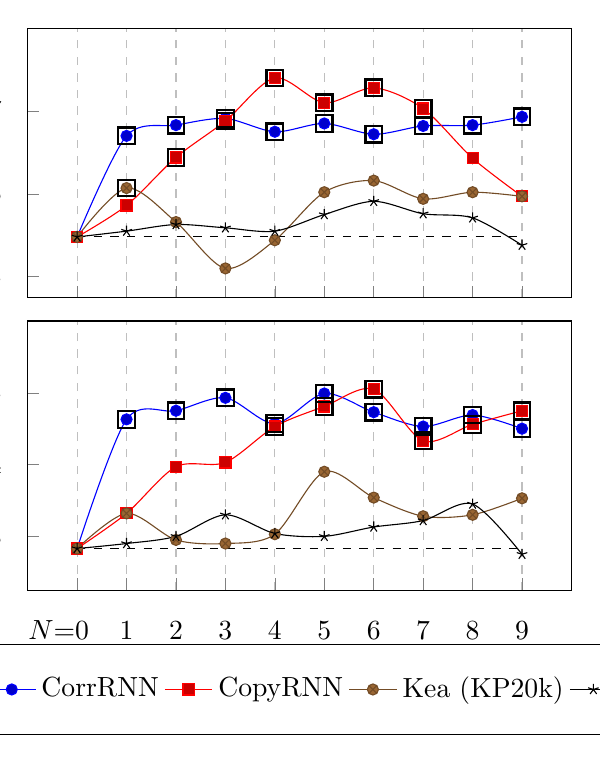
\begin{tikzpicture}[trim axis left,trim axis right]

    \begin{groupplot}[
        group style={
          group size=1 by 2,
          vertical sep=1.3cm,
        },
        width=0.7\textwidth, height=5cm,
        xmin=-1, xmax=10,
        xtick = {0, 1, 2, 3, 4, 5, 6, 7, 8, 9},
        tick pos=left,
        grid style={dashed, gray!50},
        xmajorgrids,
        legend columns=-1,
        legend style={
            anchor=north west,
            at={(-0.09,-0.2)}
        },
    ]
    
    \nextgroupplot[
        ymin=34.75, ymax=38,
        xticklabels={,,,},
        ytick = {35, 36, 37},
    ]
    \node[] at (axis cs: .4, 37.5) {{{{\small \trm}}}};

    \addplot+[smooth] plot coordinates {
        (0, 35.48) (1, 36.70) (2, 36.83) (3, 36.91) (4, 36.75) (5, 36.85) (6, 36.72) (7, 36.82) (8, 36.83) (9, 36.93)};
    \addlegendentry{CorrRNN}
    
    \addplot+[smooth] plot coordinates {
        (0, 35.48) (1, 35.86) (2, 36.44) (3, 36.88) (4, 37.40) (5, 37.10) (6, 37.28) (7, 37.03) (8, 36.43) (9, 35.97)};
    \addlegendentry{CopyRNN}

    \addplot+[smooth] plot coordinates {
        (0, 35.48) (1, 36.07) (2, 35.66) (3, 35.10) (4, 35.44) (5, 36.02) (6, 36.16) (7, 35.94) (8, 36.02) (9, 35.97)};
    \addlegendentry{Kea (KP20k)}

    \addplot+[smooth] plot coordinates {
        (0, 35.48) (1, 35.55) (2, 35.63) (3, 35.59) (4, 35.55) (5, 35.75) (6, 35.91) (7, 35.76) (8, 35.71) (9, 35.38)};
    \addlegendentry{MPRank}

    % baseline
    \addplot[mark=none, black, dashed] coordinates {(0, 35.48) (9, 35.48)};

    % significative points
    \addplot[only marks, mark=square, color=black, thick, mark size=3pt] plot coordinates {
        (2, 36.44) (3, 36.88) (4, 37.40) (5, 37.10) (6, 37.28) (7, 37.03) (1, 36.70) (2, 36.83) (3, 36.91) (4, 36.75) (5, 36.85) (6, 36.72) (7, 36.82) (8, 36.83) (9, 36.93) (1, 36.07)};
    \legend{}

    \nextgroupplot[
        yshift=1cm,
        ymin=32.25,ymax=36,
        xticklabels={$N$=0\quad~~,1, 2, 3, 4, 5, 6, 7, 8, 9},
        ytick = {32, 33, 34, 35},
    ]
    \node[] at (axis cs: .4, 35.5) {{{{\small \tr}}}};
    
    \addplot+[smooth] plot coordinates {
        (0, 32.83) (1, 34.63) (2, 34.75) (3, 34.93) (4, 34.57) (5, 34.99) (6, 34.73) (7, 34.53) (8, 34.69) (9, 34.50)};
    \addlegendentry{CorrRNN}
    
    \addplot+[smooth] plot coordinates {
        (0, 32.83) (1, 33.32) (2, 33.97) (3, 34.03) (4, 34.53) (5, 34.81) (6, 35.05) (7, 34.33) (8, 34.56) (9, 34.75)};
    \addlegendentry{CopyRNN}
    
    \addplot+[smooth] plot coordinates {
        (0, 32.83) (1, 33.32) (2, 32.95) (3, 32.90) (4, 33.03) (5, 33.90) (6, 33.54) (7, 33.28) (8, 33.30) (9, 33.53)};
    \addlegendentry{Kea (KP20k)}
    
    
    \addplot+[smooth] plot coordinates {
        (0, 32.83) (1, 32.90) (2, 33.00) (3, 33.30) (4, 33.04) (5, 33.00) (6, 33.13) (7, 33.22) (8, 33.45) (9, 32.75)};
    \addlegendentry{MPRank}
    
    
    % baseline
    \addplot[mark=none, black, dashed] coordinates {(0, 32.83) (9, 32.83)};
    
    % significative points
    \addplot[only marks, mark=square, color=black, thick, mark size=3pt] plot coordinates {
        (4, 34.53) (5, 34.81) (6, 35.05) (7, 34.33) (8, 34.56) (9, 34.75) (1, 34.63) (2, 34.75) (3, 34.93) (4, 34.57) (5, 34.99) (6, 34.73) (7, 34.53) (8, 34.69) (9, 34.50)};

    \end{groupplot}
    %\end{axis}
    
    \end{tikzpicture}
    %\end{subfigure}


    \caption{Scores de \map{} pour \textsc{Bm25}+RM3 sur NTCIR-2 en fonction du nombre $N$ de mots-clés prédits. Le symbole $\square$ indique une amélioration significative par rapport aux résultats sans mots-clés prédits.}
    \label{fig:n_vs_perf}
\end{figure}

%Explication ancien graphique
%Les gains sont peu importants pour un ou deux mots-clés prédits et conséquents à partir de 4 mots-clés.
%Néanmoins, seul CopyRNN apporte des améliorations significatives entre 3 et 9 mots-clés
%Dans la configuration \trm{}, CopyRNN est à nouveau la seule méthode qui atteint un résultat significatif tandis que les autres présentent des résultats mitigés, parfois même des scores dégradés, en particulier avec MPRank.
%L'une des explications probables est que MPRank et dans moindre mesure CorrRNN produisent des mots-clés présentant une distance sémantique avec les mots-clés de référence.
%Les résultats de CopyRNN et CorrRNN sont proches de l'optimum pour $N=5$, ce qui confirme notre choix initial pour de 5 mots-clés établis selon le critère de production moyenne de mots-clés auteurs.


% Explication nouveaux graphiques
Deux tendances distinctes s'observent dans ces graphiques: les méthodes neuronales augmentent d'au moins un point (avec au moins deux mots-clés ajoutés) et ces augmentations sont souvent significatives; les méthodes en chaîne de traitement augmentent d'un point au maximum et ne sont jamais significatives (sauf Kea dans la configuration \trm{} avec un mot-clé ajouté).
% CorrRNN
Les résultats de CorrRNN sont assez stables quel que soit le nombre de mots-clés ajoutés, le maximum étant atteint à 5 pour \tr{} et 3 pour \trm{}.
L'ajout d'un nombre important de mots-clés ne dégrade pas les performances, les mots-clés sont donc cohérents avec les documents et ce dès le premier mot-clé.
% CopyRNN
Les résultats de CopyRNN atteignent le maximum à 4 mots-clés ajoutés avec \trm{} et 6 avec \tr{}.
Les premiers mots-clés se complètent contrairement à CorrRNN dont seul le premier mot-clé est utile à \bmrm{} pour sélectionner les documents pertinents.
% MPRank
Les résultats de MPRank montrent que ses mots-clés sont peu utiles; notons une amélioration maximale de 0,5 pour 8 mots-clés ajoutés avec \tr{} et 6 avec \trm{}.
% Kea
Kea augmente significativement avec \trm{} et un mot-clé ajouté. La forte augmentation avec \tr{} et diminution avec \trm{} sont dues à RM3 car les scores pour \bm{} (non présentés ici) ne montrent pas ces fortes variations.


Les résultats de CopyRNN et CorrRNN sont proches de l'optimum pour $N=5$, ce qui confirme empiriquement notre choix initial de 5 mots-clés établis selon le critère de production moyenne de mots-clés auteurs.



\subsection{Impact du domaine sur les mots-clés prédits}\label{sub:impactdom}

Les méthodes neuronales de production de mots-clés présentent une capacité de généralisation limitée, ce qui signifie que leurs performances se dégradent sur des documents différents de ceux rencontrés lors de l'entraînement~\cite{weber_fine_2018}.
Pour quantifier l'impact de la généralisation de ces méthodes neuronales sur l'efficacité de la recherche, nous avons divisé les requêtes de NTCIR-2 en deux ensembles disjoints: \textit{en-domaine} pour celles qui appartiennent à des domaines de recherche présents dans KP20k, et \textit{hors-domaine} pour les autres.
Nous nous attendons donc à ce que l'ajout de mots-clés prédits par les méthodes supervisées ait un plus grand impact sur les scores des requêtes \textit{en-domaine} que sur les requêtes \textit{hors-domaine}.
Les requêtes ont été classées en fonction de leur contenu et du champ \texttt{<FIELD>}.
Les requêtes appartenant à une majorité de domaines présents dans KP20k\footnote{\foreign{Electricity, information and control}; \foreign{Science}; \foreign{Chemistry} et \foreign{Engineering}} sont considérées \textit{en-domaine} (27 requêtes);
et celles appartenant à une majorité des domaines non présents dans KP20k\footnote{\foreign{Biology and agriculture}; \foreign{Medicine and dentistry}; \foreign{Cultural and social science} et \foreign{Architecture, civil engineering and landscape gardening}} sont considérées \textit{hors-domaine} (22 requêtes).
Les résultats sont présentés dans le tableau~\ref{tab:ir_per_domain}.

\begin{table}[ht!]
    \centering
    \setlength{\tabcolsep}{4pt}
    \resizebox{.6\textwidth}{!}{%
    % in -> 1, 2, 5, 6
    % out -> 3, 4, 7, 8
    
    % Header 8 colonnes
    \begin{tabular}{l|c@{\hspace*{0mm}}r c@{\hspace*{0mm}}r|c@{\hspace*{0mm}}r c@{\hspace*{0mm}}r}
        % BM25+RM3 version redefining-absent-keyphrases
        \toprule
        \multirow{2}{*}{\textbf{Méthode}} & \multicolumn{4}{c|}{\tr} & \multicolumn{4}{c}{\trm}\\
        ~ & \multicolumn{2}{c}{\textbf{E}} & \multicolumn{2}{c|}{\textbf{H}} & \multicolumn{2}{c}{\textbf{E}} & \multicolumn{2}{c}{\textbf{H}} \\
        \midrule
        - & \multicolumn{2}{c}{33,1} & \multicolumn{2}{c|}{32,5} & \multicolumn{2}{c}{36,1} & \multicolumn{2}{c}{34,7} \\
        \addlinespace
        MPRank & 33,3 & \ddiff{0,2} & 32,6 & \ddiff{0,1} & 36,8 & \ddiff{0,7} & 34,4 & \ddiff{-0,3} \\
        Kea (KP20k) & 34,1 & \ddiff{1,0} & 33,7 & \ddiff{1,2} & 37,3 & \ddiff{1,2} & 34,4 & \ddiff{-0,3} \\
        \addlinespace
        CorrRNN & 34,8 & \ddiff{1,7} & \bests{35,2} & \ddiff{2,7} & 37,3 & \ddiff{1,2} & \best{36,4} & \ddiff{1,7} \\
        CopyRNN & \bests{35,5} & \ddiff{2,4} & 34,0 & \ddiff{1,5} & \bests{37,9} & \ddiff{1,8} & 36,1 & \ddiff{1,4} \\
        \bottomrule
        
        \iffalse
        % BM25
        \toprule
        \multirow{2}{*}{\textbf{Méthode}} & \multicolumn{4}{c|}{\tr} & \multicolumn{4}{c}{\trm}\\
        BM25 & \multicolumn{2}{c}{\textbf{E}} & \multicolumn{2}{c|}{\textbf{H}} & \multicolumn{2}{c}{\textbf{E}} & \multicolumn{2}{c}{\textbf{H}} \\
        \midrule
        -           & \multicolumn{2}{c}{29,5} & \multicolumn{2}{c}{29,6} & \multicolumn{2}{c}{32,9} & \multicolumn{2}{c}{30,8} \\
        MPRank      & 29,7 & \ddiff{0,1} & 29,7 & \ddiff{0,1} & 32,8 & \ddiff{-0,1} & 31,1 & \ddiff{0,3} \\
        Kea (KP20k) & \sign{31,1} & \ddiff{1,5} & 29,3 & \ddiff{-0,3} & 33,4 & \ddiff{0,6} & 30,5 & \ddiff{-0,3} \\
        CorrRNN     & \bests{32,3} & \ddiff{2,7} & \best{30,8} & \ddiff{1,3} & \best{33,7} & \ddiff{0,9} & 30,7 & \ddiff{-0,1} \\
        CopyRNN     & \sign{32,0} & \ddiff{2,4} & 30,7 & \ddiff{1,2} & 33,3 & \ddiff{0,5} & \best{31,4} & \ddiff{0,6} \\
        \bottomrule
        \fi

    \end{tabular}
    }
    \caption{Scores de \map{} sur la collection NTCIR-2 pour \textsc{Bm25}+RM3 sur les requêtes \textit{en-domaine}~(E) et \textit{hors-domaine}~(H). La différence de score avec la configuration sans mot-clés prédits est affiché en gris. Le symbole \da{} indique une amélioration significative par rapport à une indexation sans mots-clés produits automatiquement.}
    \label{tab:ir_per_domain}
\end{table}

L'examen du tableau~\ref{tab:ir_per_domain} montre que les performances sont globalement plus faibles pour les requêtes \textit{hors-domaine}.
Les faibles performances pour l'indexation sans mots-clés prédits et pour MPRank -- qui ne sont pas censés être affectés par le domaine des documents -- s'expliquent par le nombre de documents pertinents pour les requêtes des deux catégories. Les requêtes \textit{en-domaine} ont en moyenne 35 documents pertinents, tandis que les requêtes \textit{hors-domaine} en ont 21, il est donc plus difficile de trouver les documents des requêtes \textit{hors-domaine}.
Au lieu de regarder les scores, nous nous intéressons à l'augmentation des scores de \map{} (en gris) par rapport à une indexation sans mots-clés prédits (ligne \say{~-~}).
% Le R@1000 pour T+A est 78% (E) et 74% (H) donc pas de différence sur le nb de documents possible de retrouver
%
Dans la configuration \tr{} les mots-clés de MPRank et Kea améliorent autant les scores des requêtes \textit{en} et \textit{hors-domaine}, ce qui conforte notre hypothèse selon laquelle les méthodes non neuronales sont peu impactées par le domaine.
Dans la configuration \trm{} pour les requêtes \textit{hors-domaine} l'ajout des mots-clés de MPRank et Kea dégradent les scores, ce qui indique que ces mots-clés ne sont pas assez similaires aux mots-clés de référence et qu'ils font baisser l'importance des mots-clés de référence.
%
Pour CorrRNN et CopyRNN, deux méthodes supervisées neuronales, les résultats diffèrent.
L'indexation utilisant les mots-clés de CopyRNN obtient les résultats attendus, l'augmentation de score est plus élevée pour les requêtes \textit{en-domaine} que pour les requêtes \textit{hors-domaine} (2,4 contre 1,5 pour la configuration \trc{}).
Au contraire, l'augmentation des scores liés aux mots-clés de CorrRNN est meilleure pour les requêtes \textit{hors-domaine} que pour les requêtes \textit{en-domaine} (2,7 contre 1,7 pour la configuration \trc{}).
La méthode CorrRNN semble donc mieux généraliser que CopyRNN à des documents de domaines non vus durant l'entraînement.



%La méthode MPRank, qui n'est pas sensée être affectée par la dichotomie \textit{en-domaine} / \textit{hors-domaine} car elle est non supervisée, augmente les scores de manière différente selon les classes \textit{en} ou \textit{hors-domaine}.
%L'augmentation de score est plus élevée pour les requêtes \textit{hors-domaine} pour la configuration \trm{} (0,7 contre \num{-0.3})). A cause de RM3.

%Pour les méthodes neuronales CorrRNN et CopyRNN, dont la production de mots-clés devrait être impactée par le domaine des documents, l'augmentation du score de \map{} est plus élevée pour les requêtes \textit{en-domaine} que \textit{hors-domaine} sauf pour CorrRNN dans la configuration \tr{}.
%Par exemple CorrRNN avec une indexation \trm{} augmente la \map{} de 0,9 sur les requêtes \textit{en-domaine} et de 0,4 \textit{hors-domaine}.
%Cette observation conforte notre hypothèse selon laquelle les méthodes de génération de mots-clés généralisent moins bien aux documents dont les domaines ne sont pas présents dans les données d'entraînement.
%En étudiant les scores, nous remarquons que seuls les mots-clés de CopyRNN améliorent significativement l'efficacité de recherche sauf pour l'indexation \trm{} avec les requêtes \textit{hors-domaines}.
%Dans cette configuration d'indexation il est plus difficile d'obtenir une augmentation significative, en effet les mots-clés prédits ne doivent pas être redondant avec les mots-clés de référence et/ou couvrir d'autres concept du document. Pour la configuration \tr{} les mots-clés ajoutés ont seulement besoin de couvrir d'autres concepts pour augmenter les résultats.


%Cette expérience montre que l'expansion de documents à l'aide des méthodes de production de mot-clé neuronales actuelles n'est pas assez significative sans données d'entraînement dans le domaine.
%Cette expérience souligne aussi la nécessité de proposer des méthodes de génération de mots-clés qui peuvent s'adapter au domaine.

\begin{table}[!htbp]
    \centering
    \begin{tabular}{l|cc}
        \toprule
        Méthode & E & H \\
        \midrule
        MPRank & 13,2 & 21,1 \\
        Kea (KP20k) & 14,3 & 22,8 \\
        CorrRNN & 20,5 & 24,6 \\
        CopyRNN & \best{22,0} & \best{27,5} \\
        \bottomrule
    \end{tabular}
    \caption{Performances de production de mots-clés évalués grâce à la F@5 pour les documents \emph{en} et \emph{hors-domaine} de NTCIR-2. Un documents est hors-domaine s'il est pertinent pour une requête hors-domaine.}
    \label{tab:kg_intrinsic_domain}
\end{table}

Pour comparer cette évaluation extrinsèque à l'évaluation intrinsèque, nous faisons l'hypothèse que les documents pertinents pour une requête sont du même domaine que les requêtes. Ceci nous permet d'évaluer séparément les mots-clés des documents \textit{en} et \textit{hors-domaine}.
Il y a respectivement 921 et 444 documents \textit{en} et \textit{hors-domaine}, et aucun de ces documents n'est pertinent à la fois pour des requêtes \textit{en} et \textit{hors-domaine}.
%
Ainsi, nous présentons dans le tableau~\ref{tab:kg_intrinsic_domain} les performances des méthodes de production de mots-clés en fonction du domaine des documents.
Étonnamment, ce tableau montre que les mots-clés produits pour les documents \textit{hors-domaine} sont plus proches de la référence que ceux des documents \textit{en-domaine}.
Pour CopyRNN la F@5 de production de mot-clé pour les documents \textit{en-domaine} est de 22,0 et de 27,5 pour les documents \textit{hors-domaine}.
%Les signaux différents obtenus de l'évaluation intrinsèque et extrinsèque confirment l'importance de différentes stratégies d'évaluations.


\section{Mots-clés présents et absents}

Les mots-clés, suivant qu'ils apparaissent ou non dans le document, jouent un rôle différent dans l'indexation.
%Le fait que les mots-clés apparaissent ou non dans le document impacte l'indexation.
%Les mots-clés ont des effets différents sur les systèmes de recherche selon qu'ils apparaissent ou non dans le document.
Les \emph{mots-clés présents} mettent en évidence les parties importantes du document. Ils ajoutent de la redondance et ainsi améliorent la pondération du document. Les \emph{mots-clés absents} sont des nouveaux termes qui étendent le contenu du document. 
L'attribution de mots-clés absents apparaît comme attrayante: elle pourrait atténuer la discordance de vocabulaire entre les termes de la requête et ceux des documents~\cite{furnas_vocabulary_1987}, facilitant ainsi une meilleure récupération des documents pertinents.
Cette discordance de vocabulaire est d'autant plus importante que les documents sont courts. Les bibliothèques numériques scientifiques, par exemple, indexent majoritairement les notices scientifiques, et non pas les articles entiers en raison des problèmes de licence~\cite{huang_holes_2019} et des difficultés à les exploiter.
%Cependant, l'impact des mots-clés présents et absents sur l'amélioration de l'efficacité de la recherche n'a pas été étudié en profondeur et la définition de ce qui fait un mot-clés absent ou présent n'a pas été définie de manière précise et rigoureuse.

\begin{figure}[ht]
    \centering
    %\centerfloat
    \resizebox{0.98\textwidth}{!}{%
    \begin{tabular}{|p{1.3\textwidth}|}
%\begin{mdframed}[backgroundcolor=blue!2, font=\small]
\textbf{Study on the Structure of Index Data for \colorbox{c1}{Metasearch} \colorbox{c3}{System}}

\vspace{.9em}

This paper proposes a new technique for \colorbox{c1}{Metasearch} \colorbox{c3}{system}, which is based on the grouping of both keywords and URLs.
This technique enables \colorbox{c1}{metasearch} \colorbox{c3}{systems} to \colorbox{c5}{share} \colorbox{c4}{information} and to reflect the estimation of \colorbox{c6}{users'} preference.
With this \colorbox{c3}{system}, \colorbox{c6}{users} can search not only by their own keywords but by similarity of HTML documents.
In this paper, we describe the principle of the grouping technique as well as the summary of the existing \colorbox{c2}{search} \colorbox{c3}{systems}.

\vspace{1.1em}

\textbf{Mots-clés présent}:
\colorbox{c1}{Metasearch} --
\colorbox{c2}{Search} \colorbox{c3}{System}

\vspace{.7em}

\textbf{Mots-clés absent}:
\colorbox{c4}{Information} \colorbox{c5}{Sharing} --
\colorbox{c4}{Information} Retrieval --
\colorbox{c6}{User}'s Behavior --
Retrieval Support

\vspace{.2em}

%{\small
%\hspace{1.9cm} $\lfloor$ \hspace{.7cm} \underline{R}eordered \hspace{.6cm} $\rfloor$
%\hspace{0.1cm} $\lfloor$ \hspace{1.05cm} \underline{M}ixed \hspace{1.05cm} $\rfloor$
%\hspace{0.1cm} $\lfloor$ \hspace{.6cm} \underline{M}ixed \hspace{.6cm} $\rfloor$
%\hspace{0.1cm} $\lfloor$ \hspace{.6cm} \underline{U}nseen \hspace{.6cm} $\rfloor$
%}

%\textcolor{gray}{
%\hspace{1.9cm} \hspace{.9cm} \underline{R}éordonné \hspace{.9cm}
%\hspace{0.1cm} \hspace{.7cm} \underline{M}ixte \hspace{.7cm}
%\hspace{0.1cm} \hspace{.7cm} \underline{M}ixte \hspace{.7cm}
%\hspace{0.1cm} \hspace{.5cm} \underline{N}on-vu \hspace{.5cm}
%}

%\end{mdframed}
\end{tabular}
}
\caption{Exemple de document de la collection de test de NTCIR-2 (id: gakkai-e-0001384947).} %Les mots-clés auteur présent et absent ont été identifié selon la définition donnée dans ce document. %Les catégories fines (i.e.~\underline{R}éordonné, \underline{M}ixte et \underline{N}on-vu) sont explicitées.}
\label{fig:example_prmn}
\end{figure}

\iffalse
\begin{figure}[ht]
\begin{mdframed}[backgroundcolor=blue!2, font=\small]

\textbf{\colorbox{c3!60!60!white}{Rapid} \colorbox{c6!60!60!white}{Full-Text} \colorbox{c1!60!60!white}{Retrieval} Method with Coding \colorbox{c4!60!60!white}{Character} of \colorbox{c6!60!60!white}{Full-Text} Using both an Attribute and \colorbox{c4}{Character} \colorbox{c5}{Location}}

\vspace{.9em}

This paper describes \colorbox{c3}{rapid} \colorbox{c6}{full-text} \colorbox{c1}{retrieval} method with software and the result of retrieval-experiment. Generally in Japanese document,same Kanji \colorbox{c4!60!60!white}{character} rarely appeares and also same Kanji \colorbox{c2}{string} rarely appeares. This method uses these characteristics of Japanese document. We are able to rapidly \colorbox{c1}{retrieval} \colorbox{c6}{full-text} with this method.

\say{\texttt{[...] and \colorbox{c4}{Character} \colorbox{c5}{Location}}}
\say{\texttt{[...] rapidly \colorbox{c1}{retrieval} \colorbox{c6}{full-text} with [...]}}
\say{\texttt{[...]  [...]}}
\say{\texttt{[...]  [...]}}


\vspace{1.1em}

\textbf{Mots-clés présent}:
\colorbox{c6}{Full-text}~\colorbox{c1}{Retrieval} -- \colorbox{c4}{Character}~\colorbox{c5}{Location}

\vspace{.7em}

\textbf{Mots-clés absent}:
\colorbox{c4}{Character}~\colorbox{c2}{String} -- \colorbox{c3}{Rapid}~\colorbox{c1}{Retrieval} -- Information~\colorbox{c1}{Retrieval} -- \\
\phantom{\textbf{Mots-clés absent}:} Character-string~Collation



\end{mdframed}
\caption{Exemple de document de la collection de test de NTCIR-2 (id: gakkai-e-0000056172).} %Les mots-clés auteur présent et absent ont été identifié selon la définition donnée dans ce document. %Les catégories fines (i.e.~\underline{R}éordonné, \underline{M}ixte et \underline{N}on-vu) sont explicitées.}
\label{fig:example_prmn}
\end{figure}
\fi

Bien que cela ne soit pas indiqué explicitement, les travaux sur les mots-clés adoptent la définition de~\citet{meng_deep_2017} dans laquelle les mots-clés qui ne correspondent à aucune sous-séquence contiguë du texte source sont considérés comme absents.
Du point de vue de la recherche d'information, où les mots pleins racinisés sont utilisés pour indexer les documents, cette définition n'est pas suffisamment explicite comme le montre l'exemple de la figure~\ref{fig:example_prmn}.
Nous voyons que, selon cette définition, certains mots-clés absents peuvent avoir tous leurs mots dans le document source, et donc agir comme des mots-clés présents lors de l'indexation.
Seule une fraction des mots qui composent ces mots-clés absents étendent véritablement le document, qui dans notre exemple est l'ensemble de mots $\lceil$\emph{retrieval}, \emph{behavior}, \emph{support}$\rfloor$.
Du point de vue de la génération de mots-clés, la définition de~\citet{meng_deep_2017} n'est pas non plus entièrement satisfaisante.
En effet, les modèles génératifs sont entraînés à générer des mots à partir d'un vocabulaire ou à copier des mots à partir du document source.
L'utilisation de modèles génératifs est peut-être disproportionnée, une grande partie des mots-clés de référence sont présents dans le document et peuvent donc être copiés (voir section~\ref{sec:benchmark_datasets}).
% extracted
Nous soutenons ici que la place trop importante que les modèles neuronaux donnent à la génération de mot-clés est l'une des raisons de leur faible performance. %~\cite{gallina_large-scale_2020}.
Nous allons discuter la définition actuelle des mots-clés absents et proposer une catégorisation des mots-clés absents en adéquation avec la RI qui nous permettra d'étudier plus finement l'impact des mots-clés absents et présents pour la RI.



\subsection{Redéfinir les mots-clés absents}
\label{sec:def}

La définition usuelle des mots-clés présents et absents a été proposée par~\citet{meng_deep_2017} comme suit:
\say{\emph{nous désignons les phrases qui ne correspondent à aucune sous-séquence contiguë du texte source comme des mots-clés absents et celles qui correspondent entièrement à une partie du texte comme des mots-clés présents}}.\footnote{\say{we denote phrases that do not match any contiguous subsequence of source text as absent keyphrases, and the ones that fully match a part of the text as present keyphrases}}
Nous soutenons que cette définition n'est pas assez précise pour deux raisons.
Tout d'abord, les pré-traitements à appliquer pour faire correspondre le mot-clé et le texte ne sont pas explicités, cette étape est donc à la discrétion de l'implémentation.
Ensuite, la définition de l'absence d'un mot-clé englobe ici plusieurs phénomènes distincts (occurrence totale, occurrence partielle, pas d'occurrence du mot-clé dans le document).
% Distinguer les mots-clés absents et présents n'est pas aussi simple qu'il y parait.

% Mise en correspondance
Pour identifier si un mot-clé est une \say{sous-séquence contiguë du texte source} il est évident qu'une simple correspondance de chaîne de caractères n'est pas acceptable car elle produit des faux positifs (par ex. \texttt{supervised learning} est une sous-séquence contiguë de  \texttt{\underline{\textcolor{gray}{un}}supervised learning}).
Le mot-clé et le document doivent donc être mis en correspondance au niveau des mots mis en minuscules.
La racinisation doit aussi être appliquée pour traiter une partie des variantes morphologiques des mots. Ce traitement est standard dans l'indexation de documents pour la RI ainsi que pour l'évaluation des méthodes de production de mots-clés.

%À partir de la définition de~\citet{meng_deep_2017}, \say{\emph{nous désignons les phrases qui ne correspondent à aucune sous-séquence contiguë du texte source comme des mots-clés absents et celles qui correspondent entièrement à une partie du texte comme des mots-clés présents}}\footnote{\say{we denote phrases that do not match any contiguous subsequence of source text as absent keyphrases, and the ones that fully match a part of the text as present keyphrases}}, il est évident qu'une simple correspondance de chaîne de caractères entre les mots-clés et le document source n'est pas acceptable car elle produit des faux positifs (par ex. par exemple, \say{\emph{supervised learning}} correspond à \say{\emph{\textcolor{gray}{un}supervised learning}}).
%L'utilisation de la racinisation permet d'infléchir cette contrainte de correspondance et de traiter une partie des variantes morphologiques d'un mot.
%La racinisation est d'ailleurs une  procédure standard dans l'indexation des documents pour la RI mais aussi dans l'évaluation des méthodes de génération de mots-clés par rapport à l'annotation de référence~\cite{hasan_automatic_2014}.

\iffalse
\begin{figure}[ht!]
    \centering
    \inputminted[fontsize=\footnotesize]{python}{6_impact_ri/figures/code_prmu.py}
    \caption{Code python calculant les catégories fine PRMN d'un mot-clé (\texttt{kw}) étant donné un document (\texttt{doc}).}
    \label{fig:finer_category_code}
\end{figure}
\fi

% Définition d'absence
L'\say{absence} de mots-clés recoupe plusieurs phénomènes que nous divisons en trois sous-catégories selon la proportion de mots présents qu'ils contiennent.
La figure~\ref{fig:example_prmn} présente un exemple de ces trois sous-catégories.
%Sur l'exemple de la figure~\ref{fig:example_prmn}, les mots-clés absents peuvent être divisés en trois sous-catégories selon la proportion de mots présents qu'ils contiennent.
Certains mots-clés absents ont une partie, voire la totalité, de leurs mots (dans des formes racinées) présents dans le texte tandis que d'autres ne comportent que des mots absents du texte.
% Présentation de notre catégorisation
Nous proposons donc une catégorisation plus fine, nommée PRMN, illustrée par l'exemple de la figure~\ref{fig:example_prmn}:


\begin{itemize}[wide=0.5em,leftmargin=1em,itemsep=0.05em,font=\bfseries]
    \item[\present:] mot-clé dont tous les mots apparaissent de manière contiguë et dans le même ordre que dans le texte. Par exemple \say{\colorbox{c2}{Search} \colorbox{c3}{System}} et \say{\texttt{[...] existing \colorbox{c2}{search} \colorbox{c3}{systems}.}}.
    
    \item[\reordonne:] mot-clé dont tous les mots apparaissent dans le texte mais pas de manière contiguë et/ou dans un ordre différent. Par exemple \say{\colorbox{c4}{Information} \colorbox{c5}{Sharing}} et \say{\texttt{[...]to \colorbox{c5}{share} \colorbox{c4}{information} and [...]}} ou encore le mot-clé \say{\colorbox{c2}{Search} \colorbox{c3}{System}} dont les deux mots apparaissent aussi de manière non contiguë.
    
    \item[\mixte:] mot-clé dont certains mots (mais pas tous) apparaissent dans le texte. Par exemple \say{\colorbox{c4}{Information} Retrieval} et \say{\texttt{[...] to \colorbox{c5}{share} information and [...]}}, le mot \say{Retrieval} n'apparaît pas dans le texte.
    
    \item[\nonvu:] mot-clé dont aucun mot n'apparaît dans le texte. Par exemple \say{Retrieval Support}.
\end{itemize}

Contrairement à la classification binaire (c.-à-d. présent ou absent) de \citet{meng_deep_2017}, notre schéma de catégorisation établit une distinction entre les catégories de mot-clés qui étendent le document (\mixte{} et \nonvu) et celles qui ne l'étendent pas (\present{} et \reordonne).
Notons que cette définition peut être affinée en séparant les mots-clés \reordonnes{} dont les mots apparaissent de manière contiguë et les autres. % Nous pourrions aussi ne pas prendre en compte les mots-vides pour cette correspondance.

L'utilisation de cette catégorisation va nous permettre d'établir la contribution de chaque catégorie à l'efficacité de la recherche d'articles scientifiques.
De plus, ce schéma fournit un nouvel éclairage pour évaluer la capacité des méthodes de génération de mots-clés à produire des mots-clés absents en comparant leurs distributions PRMN à celles observées dans les annotations de référence.
En d'autres termes, pour être performante, une méthode doit imiter la distribution des mots-clés absents dans l'annotation manuelle.


\subsection{Distribution des mots-clés de référence}
\label{sec:dist}

Nous étudions maintenant les mots-clés de référence selon la classification PRMN pour avoir une vision plus précise du nombre de mots-clés qui étendent les documents.

\begin{table}[!hbt]
    \centering
    \begin{tabular}{l|rrrr|r}
    %\cline{4-5}
    %\multicolumn{3}{c}{~} &
    %\multicolumn{2}{|c|}{~\hfill {\scriptsize doc. expansion} \hfill~}
    %\multicolumn{2}{@{}c@{}}{\small{$\lceil$ \hfill {\scriptsize doc. expansion} \hfill $\rceil$}}
    %\\ %[+.1cm]
    %\cline{3-5}
    \multicolumn{2}{c}{~} &
    \multicolumn{3}{c}{\small{$\lceil$ \hfill {\scriptsize mots-clés absents} \hfill $\rceil$}}
    \\
    %\multicolumn{1}{c}{~} &
    %\multicolumn{2}{c@{}}{\small{$\lceil$ \hfill {\scriptsize term-weighting} \hfill $\rceil$}} &
    %\multicolumn{2}{c}{\small{$\lceil$ \hfill {\scriptsize doc. expansion} \hfill $\rceil$}} \\
    \toprule
    \textbf{Données}  & \textbf{\%P} & \textbf{\%R} & \textbf{\%M} & \textbf{\%N} & \textbf{\%ma} \\
    \midrule
     NTCIR-2 & 61,9 &  8,1 & 16,5 & 13,5 & 21,4 \\
     ACM-CR  & 53,6 & 11,7 & 19,3 & 15,4 & 25,5 \\
     KP20k   & 60,2 &  9,5 & 15,4 & 15,0 & 22,3 \\
     %KDD     & 50,7 &  9,4 & 20,7 & 19,2 & 29,4 \\
     %WWW     & 46,6 &  9,6 & 20,9 & 23,0 & 32,5 \\
    \bottomrule
    %\multicolumn{1}{c}{~} &
    %\multicolumn{2}{c@{}}{\small{$\lfloor$ \hfill {\scriptsize pond. des termes} \hfill $\rfloor$}} &
    %\multicolumn{2}{c}{\small{$\lfloor$ \hfill {\scriptsize expansion de doc.} \hfill $\rfloor$}}
    \end{tabular}
    \caption{Proportion de mots-clés \presents{}, \reordonnes{}, \mixtes{} et \nonvus{} dans les jeux de données. Nous rapportons aussi le pourcentage de mots unique absents qui proviennent des mots-clés M et N (\%ma).}
    \label{tab:prmu_dist_ref}
\end{table}
%|      102411 |      70734 | 53.6 | 11.7 | 19.3 | 15.4 | 13.4 |  4.5 |

% Results computed on the 24-03-2021 using https://gist.github.com/ygorg/887e46c68d74c3c90eef0893284a6c72
%     NTCIR-2 & 61.2 &  8.2 & 16.6 & 14.1 & 21.6 \\
%     ACM-CR  & 61.3 & 10.3 & 15.3 & 12.8 & 22.8 \\
%     KP20k   & 61.0 &  9.7 & 15.7 & 13.7 & 22.2 \\
%     %KDD     & 50.8 &  9.4 & 20.7 & 19.1 & 30.0 \\
%     %WWW     & 57.8 &  7.6 & 16.5 & 18.2 & 30.4 \\

Le tableau~\ref{tab:prmu_dist_ref} montre la proportion de mots-clés de référence attribués par les auteurs pour chaque catégorie dans nos collections de test NTCIR-2 et ACM-CR.
Nous présentons aussi à titre de comparaison le jeu de données KP20k~\cite{meng_deep_2017} utilisé pour entraîner les modèles neuronaux de génération de mots-clés.

Nous observons des distributions similaires dans les différents ensembles de données: les mots-clés absents représentent environ \npercent{40} du nombre total de mots-clés.
ACM-CR présente le ratio de mots-clés \present{} le plus faible (\npercent{53.6}) et les pourcentages les plus élevés de mots-clés \reordonnes{} (\npercent{11.7}) et \mixtes{} (\npercent{19.3}).
Les distributions PRMN de NTCIR-2 et KP20k sont similaires; KP20k comporte néanmoins \npercent{15.0} de mots-clés \nonvu{} alors que NTCIR-2 n'en comporte que \npercent{13.5}.
La plupart des mots-clés absents (selon la définition de Meng) appartiennent aux catégories \mixtes{} et \nonvus{}.

Pour avoir une idée précise du nombre de nouveaux mots ajoutés lors de l'indexation des mots-clés absents, nous calculons le ratio de mots uniques absents du document (\%ma) qui proviennent des mots-clés. %\mixte{} ou \nonvu.
Nous constatons que seulement $1/4$ des mots uniques composants les mots-clés étendent les documents.
Pourtant, comme nous le verrons plus loin, cette petite fraction de mots nouveaux est à l'origine d'une grande partie des gains observés dans l'efficacité de la recherche.



\subsection{Impact des mots-clés de référence}
\label{sec:ir}

Après avoir étudié la distribution des mots-clés de référence selon la catégorisation PRMN, nous étudions dans cette expérience l'impact sur la RI de ces différentes catégories.
Pour cela, nous utilisons comme base de comparaison l'indexation du titre et du résumé des documents (\trc{}) puis indexons les différentes catégories de mots-clés PRMN.
Nous comparons donc chaque catégorie individuellement mais aussi les mots-clés \presents{} et \reordonnes{} qui n'ajoutent pas de nouveaux mots au document, les mots-clés \mixtes{} et \nonvus{} qui étendent le document avec de nouveaux mots et enfin les mots-clés absents (\reordonnes{}, \mixtes{} et \nonvus).

Le tableau~\ref{tab:prmu_ref} présente les résultats des systèmes de recherche sur ces documents enrichis avec ces différents ensembles de mots-clés.
Nous constatons que l'ajout de mots-clés améliore toujours l'efficacité de recherche pour NTCIR-2 et seulement avec \bm{} pour ACM-CR.
Un examen plus poussé révèle que les gains les plus importants sont obtenus avec les mots-clés \mixtes{} et \nonvus{}:
pour NTCIR-2, les scores maximaux sont atteints grâce aux mots-clés \mixtes{} (30,8 pour \bm{} et 33,9 pour \bmrm{});
pour ACM-CR, ils sont atteints avec les mots-clés \nonvus{} (36,2 et 33,8).

\iffalse
\begin{table*}[ht!]
    \centering
    \begin{tabular}{l|ccc||ccc}
        \multicolumn{1}{c}{} & \multicolumn{3}{c}{$\lceil$ \hfill NTCIR-2 (\map{}) \hfill $\rceil$} & \multicolumn{3}{c}{$\lceil$ \hfill ACM-CR (R@10) \hfill $\rceil$}\\
        \toprule
        \textbf{index} & \textbf{\textsc{Bm25}} & \textbf{+RM3} & \textbf{\#mc} & \textbf{\textsc{Bm25}} & \textbf{+RM3} & \textbf{\#mc}\\
        %\cmidrule(lr){2-3} \cmidrule(lr){4-5}
        %~ & \map & P10 & \map & P10 \\
        \midrule
            \trc   & 29,6 & 32,8 & - & 35,6 & 34,1 & - \\
        \cmidrule(lr){1-7}
            ~+~\present   & \sign{30,7} & 33,5 & 2,9 & 36,0 & 34,1 & 2,4 \\
            ~+~\reordonne & 29,8 & 33,5 & 0,4  & 35,4 & 33,4 & 0,5 \\ %C1
            ~+~\mixte     & \bests{30,8} & \best{33,9} & 0,8 & \best{36,2} & 33,4 & 0,9 \\ %C2
            ~+~\nonvu     & 29,7 & \best{33,9} & 0,7 & \best{36,2} & \best{33,8} & 0,8 \\ % C3
        \cmidrule(lr){1-7}
            ~+~Pond. \scriptsize{(P+R)}    & \sign{30,6} & 33,8 & 3,3  & 35,8 & 32,4 & 2,9\\ % P+C1
            ~+~Exp. \scriptsize{(M+N)}     & \bests{30,8} & \best{34,3} & 1,5 & \best{37,2} & \best{33,4} & 1,6\\ % C2+C3
        \cmidrule(lr){1-7}
            ~+~Absent \scriptsize{(R+M+N)} & \sign{30,8} & \sign{34,9} & 1,9 & 36,6 & 34,1 & 2,1 \\ % abs
         \cmidrule(lr){1-7}
            ~+~P+R+M+N    & \signn{\sign{31,9}}  & \signn{\sign{35,5}}   & 4,8  & 36,7 & 32,9 & 4,5\\
         \bottomrule
    \end{tabular}
    \caption{Efficacité de la recherche de \textsc{Bm25} et \textsc{Bm25}+RM3 en utilisant différentes configurations d'indexation. Nous rapportons aussi le nombre moyen de mots-clés (\#mc). \da et \dda indiquent la significativité par rapport à, respectivement, l'indexation titre \& résumé et \underline{P}résent.}
    \label{tab:prmu_ref}
\end{table*}
\fi


\begin{table*}[ht!]
    \centering
\begin{tabular}{l|c@{\hspace*{0mm}}rc@{\hspace*{0mm}}rc||c@{\hspace*{0mm}}rc@{\hspace*{0mm}}rc}
    \multicolumn{1}{c}{} & \multicolumn{5}{c}{$\lceil$ \hfill NTCIR-2 (\map{}) \hfill $\rceil$} & \multicolumn{5}{c}{$\lceil$ \hfill ACM-CR (R@10) \hfill $\rceil$}\\
        \toprule
index    & \multicolumn{2}{l}{\bm} & \multicolumn{2}{l}{+RM3} & \textbf{\#mc} & \multicolumn{2}{l}{\bm} & \multicolumn{2}{l}{+RM3} & \textbf{\#mc} \\
\midrule
\trc    & \multicolumn{2}{c}{29,6} &  \multicolumn{2}{c}{32,8} &  - & \multicolumn{2}{c}{35,6} &     \multicolumn{2}{c}{34,1} &    - \\
\cmidrule(lr){1-11}
~+~\present     &  \sign{30,7} &  \diff{1,2} &         33,5 &  \diff{0,6} &  2,9 &
                          36,0 &  \diff{0,4} &         34,1 & \diff{-0,0} &  1,6 \\
~+~\reordonne   &         29,8 &  \diff{0,2} &         33,5 &  \diff{0,6} &  0,4 &
                          35,4 & \diff{-0,2} &         33,4 & \diff{-0,7} &  0,3 \\
~+~\mixte       & \bests{30,8} &  \diff{1,2} &  \best{33,9} &  \diff{1,0} &  0,8 &
                   \best{36,2} &  \diff{0,6} &         33,4 & \diff{-0,7} &  0,6 \\
~+~\nonvu       &         29,7 &  \diff{0,1} &  \best{33,9} &  \diff{1,1} &  0,7 &
                   \best{36,2} &  \diff{0,6} &  \best{33,8} & \diff{-0,3} &  0,5 \\
\cmidrule(lr){1-11}
Pond. (P+R)     &  \sign{30,6} &  \diff{1,1} &         33,8 &  \diff{1,0} &  3,3 &
                          35,8 &  \diff{0,2} &         32,4 & \diff{-1,7} &  2,0 \\
Exp. (M+N)      & \bests{30,8} &  \diff{1,3} &  \best{34,3} &  \diff{1,5} &  1,5 &
                   \best{37,2} &  \diff{1,6} &  \best{33,4} & \diff{-0,7} &  1,1 \\
\cmidrule(lr){1-11}
Absent (R+M+N)  &  \sign{30,8} &  \diff{1,2} &  \sign{34,9} &  \diff{2,0} &  1,8 &
                          36,6 &  \diff{1,0} &         34,1 &  \diff{0,0} &  1,5 \\
\cmidrule(lr){1-11}
~+~P+R+M+N &\signn{\sign{31,9}}& \diff{2,3}&\signn{\sign{35,5}}& \diff{2,7}& 4,7 &
                          36,7 &  \diff{1,1} &         32,9 & \diff{-1,2} &  3,1 \\
\bottomrule
\end{tabular}

    \caption{Efficacité de recherche de \bm{} et \bmrm{} en utilisant différentes configurations d'indexation. Est aussi indiqué le nombre moyen de mots-clés ajoutés (\#mc). Les symboles \da{} et \dda{} indiquent une amélioration significative par rapport à, respectivement, l'indexation \trc{} et \present{}.}
    \label{tab:prmu_ref}
\end{table*}


%\todo{Diviser par le nb de doc avec des mots-clés au lieu de tout les docs? Sinon modifier le tableau 6.10 6.7 6.1}

Les mots-clés qui étendent le document (ligne \say{Exp.}) sont bien plus impactants que les mots-clés qui améliorent la pondération (ligne \say{Pond.}).
 Les scores d'efficacité de recherche en fonction du nombre de mots-clés ajoutés montrent que l'ajout de 1,5 mots-clés M et N augmente plus que l'ajout de 3,3 mots-clés \presents{} et \reordonnes{} pour \bm{} et \bmrm{}.
Ce schéma d'augmentation se retrouve pour ACM-CR avec \bm{}.
%
Cette observation, et le fait que le nombre de mots-clés qui étendent le document  (ligne \say{Exp.}) est comparativement faible (moins d'un en moyenne), démontre que l'expansion des documents est plus efficace que la mise en avant des mots importants du document.
%Plus haut
Cette conclusion est confirmée par les scores plus élevés en ajoutant les mots-clés \mixtes{} et \nonvus{} (34,3) qu'en ajoutant les mots-clés \presents{} et \reordonnes{} (33,8).

% on l'a déjà vu avant pour ntcir-2
De manière surprenante, pour ACM-CR, la combinaison de l'expansion de requête (+RM3) et  l'ajout de mots-clés entraînent une baisse des résultats.
Cette baisse peut s'expliquer par le bruit que contiennent les requêtes. %(expliqué plus en détail dans la section~\ref{sub:ir_collections}).
En effet, les requêtes de cette collection sont des paragraphes extraits d'articles scientifiques qui peuvent ne pas suffisamment circonscrire la recherche. 
Dans l'exemple de la figure~\ref{fig:acmcr_topic_example}, les documents recherchés pertinents portent sur les méthodes à base de graphe et les plongements de mots. Les requêtes expriment ces sujets mais abordent aussi d'autres thématiques comme les systèmes de recherche d'information.
L'expansion de requête peut donc facilement faire dériver la requête originale vers ces autres sujets.
La baisse des résultats d'ACM-CR peut aussi être expliquée par l'incomplétude des jugements de pertinence.
Certains articles retournés répondent au besoin d'informations mais ne font pas partie des jugements de pertinence. En effet, de par la création automatique de cette collection, les jugements de pertinence incluent seulement les articles cités dans le document mais n'incluent pas les documents pertinents qui ne sont pas cités.
%L'ajout de mots-clés avec ACM-CR et \bmrm{} entraîne aussi une baisse  des scores de R@10 sauf pour l'ajout des mots-clés \presents{} et des mots-clés Absents (RMN).
%Néanmoins cette baisse, moins importante pour \say{Exp.} que pour \say{Pond.}, souligne de nouveau la meilleure efficacité de l'expansion par rapport à la pondération.

%A mettre dans une section de la conclusion et discussion sur les jeux de données
%thèse exprimentale sur des jeux de données que penses-tu de ces jeux de données ?
%pourrait-on les améliorer  actuellement thématique de recherche 
%Pour pallier l'incomplétude des jugements de pertinence, l'utilisation d'une métrique de probabilité de co-citation comme dans~\cite{livne_citesight_2014} pourrait changer ces résultats. 


\subsection{Impact des mots-clés générés présents et absents}
\label{sec:kg}

Dans cette dernière expérience, nous examinons les mots-clés générés par les méthodes neuronales selon le schéma PRMN.
Nous nous intéressons d'abord à la distribution de ces mots-clés selon la catégorisation PRMN puis à l'impact de ces mots-clés sur la RI.

\begin{table}[!ht]
    \centering
    \begin{tabular}{l|rrrr|r}
    \toprule
    \textbf{Modèle} & \textbf{\%P} & \textbf{\%R} & \textbf{\%M} & \textbf{\%N} & \textbf{F@5} \\
    \midrule
        CorrRNN & 89,7 &  7,1 &  2,5 &  0,8 & 22,1\\
        CopyRNN & 96,9 &  1,3 &  0,9 &  0,9 & 24,0\\
    %\midrule
    %    Gold & 60,2 &  9,5 & 15,4 & 15,0  \\
    \bottomrule
    \end{tabular}
    \caption{Proportion de mots-clés \underline{P}résent, \underline{R}éordonné, \underline{M}ixte et \underline{N}on-vu dans les 5 meilleurs mots-clés sur le jeu de donnée NTCIR-2. La F@5 est calculée sur les mots-clés de référence.}
    \label{tab:prmu_dist_pred_ntcir2}
\end{table}


Le tableau~\ref{tab:prmu_dist_pred_ntcir2} montre les distributions sur les catégories PRMN pour nos deux méthodes neuronales: \emph{CopyRNN} et \emph{CorrRNN} (détaillées dans le chapitre~\ref{chap:kw_production}).
Nous observons que les mots-clés prédits sont en grande majorité \presents{} et que les méthodes neuronales ont donc du mal à produire des mots-clés comportant des mots absents du document (\npercent{3.3} pour les \mixtes{} et \nonvus{} de CorrRNN).

%\subsection{Mots-clés présents et absents générés}

% La précision est mieux que le rappel: les mots-clés présent sont bien trouvé mais les absent pas du tout
D'après nos expériences présentées dans la section~\ref{sub:impactdom} (voir tableau~\ref{tab:ir_results}), l'extraction non supervisée de mots-clés n'améliore pas de manière significative l'efficacité de la recherche. La méthode MPRank dégrade même parfois les scores.
\`A l'inverse, les méthodes neuronales augmentent significativement les scores.
Cette augmentation peut être due à leur capacité à produire des mots-clés absents.
Pour vérifier cette hypothèse, nous évaluons séparément l'impact des mots-clés présents (\presents{} et \reordonnes{}) et absents (\mixtes{} et \nonvus{}) avec les méthodes neuronales CopyRNN et CorrRNN et les configurations \tr{} et \trm{}.
Nous nous attendons à ce que l'ajout des mots-clés prédits absents augmentent plus les scores que l'ajout des mots-clés présents. Ce résultat conforterait nos résultats de la section~\ref{sub:ri_impact_pred} qui montraient que les mots-clés de référence \mixtes{} et \nonvus{} étaient responsables de la majorité des gains de scores.

%\iffalse
\begin{table}[ht!]
    \centering
    \setlength{\tabcolsep}{5pt}
    \begin{tabular}{l|cc|cc}
        \toprule
        %\multirow{2}{*}{\textbf{Méthode}} & \multicolumn{2}{c|}{$T$+$R$ {\small(cf.~31,9)}} & \multicolumn{2}{c}{$T$+$R$+$M$ {\small(cf.~35,2)}}\\
        \multirow{2}{*}{\textbf{Méthode}} & \multicolumn{2}{c|}{\tr} & \multicolumn{2}{c}{\trm}\\
        ~ & \textbf{pres.} & \textbf{abs.} & \textbf{pres.} & \textbf{abs.} \\
        \midrule
        - & \multicolumn{2}{c|}{31,9} & \multicolumn{2}{c}{35,2} \\
        CorrRNN & 33,0 & 32,0 & 36,1 & 34,8 \\
        CopyRNN & \bests{34,2} & 32,1 & \bests{36,3} & 35,0 \\
        \bottomrule
    \end{tabular}
    \caption{Scores de \map pour BM25+RM3 sur NTCIR1+2 en utilisant les 5 meilleurs mots-clés absent ou présent. La première ligne indique les résultats sans mots-clés prédits. $\dagger$ indique la significativité par rapport à une indexation sans mots-clés prédits.}
    \label{tab:ir_prs_abs}
\end{table}
\fi

\begin{table}[ht!]
    \centering
    \setlength{\tabcolsep}{5pt}
    \begin{tabular}{l|cc|cc}
        \toprule
        \multirow{2}{*}{\textbf{Méthode}} & \multicolumn{2}{c|}{\tr} & \multicolumn{2}{c}{\trm}\\
        ~ & \textbf{pres.} & \textbf{abs.} & \textbf{pres.} & \textbf{abs.} \\
        \midrule
        -       & \multicolumn{2}{c|}{32.8} & \multicolumn{2}{c}{35.5} \\
        CorrRNN & \sign{34.9} & 33.0 & \sign{36.9} & 35.4 \\
        CopyRNN & \sign{34.5} & 32.6 & \sign{36.7} & 35.4 \\
        \bottomrule
    \end{tabular}
    \caption{\textcolor{red}{Version redefining} Scores de \map pour BM25+RM3 sur NTCIR1+2 en utilisant les 5 meilleurs mots-clés absent ou présent. La première ligne indique les résultats sans mots-clés prédits. $\dagger$ indique la significativité par rapport à une indexation sans mots-clés prédits.}
    \label{tab:ir_prs_abs}
\end{table}
\begin{table}[!ht]
    \centering

\begin{tabular}{l|c@{\hspace*{0mm}}rc|c@{\hspace*{0mm}}rc||c}
\toprule
 & \multicolumn{3}{c|}{\tr} & \multicolumn{3}{c||}{\trm} & \multirow{2}{*}{F@5} \\
 & \multicolumn{2}{c}{\map} & \#mc & \multicolumn{2}{c}{\map} & \#mc \\
\midrule
-     & \multicolumn{2}{c}{32,8} & 0,0 &
        \multicolumn{2}{c}{35,5} & 4,8 \\
\addlinespace
CorrRNN &
    \bests{35,0} & \diff{2,2} &    5,0 &
    \bests{36,9} & \diff{1,4} &    9,7 & 22,1 \\ % ltsj 
%(normalement ça devrait etre 22,3)
\quad Pond. \scriptsize{(P+R)} &
     \sign{34,6} & \diff{1,8} &    5,0 &
            36,7 & \diff{1,2} &    9,7 & 25,5 \\
\quad Exp. \scriptsize{(M+N)} &
            33,4 & \diff{0,6} &    1,9 &
            35,8 & \diff{0,3} &    5,2 & \pad{0}1,7 \\
\addlinespace
CopyRNN &
     \sign{34,8} & \diff{2,0} &    5,0 &
     \sign{37,1} & \diff{1,6} &    9,7 & 24,0 \\
%(normalement ça devrait être 23,9)
\quad Pond. \scriptsize{(P+R)} &
    \bests{35,0} & \diff{2,2} & 5,0 &
    \bests{37,5} & \diff{2,0}  &    9,7 & 27,6 \\
\quad Exp. \scriptsize{(M+N)}  &
            32,2 & \diff{-0,6} &    3,2 &
            34,5 & \diff{-1,0} &    6,8 & \pad{0}0,7\\
\bottomrule
\end{tabular}

    \caption{Scores de \map{} sur la collection NTCIR-2 pour \textsc{Bm25}+RM3 dans les configurations \tr{} et \trm{}. Le symbole \da{} indique une amélioration significative par rapport à l'indexation \tr{}. \say{Pond.} dénote l'ajout des mots-clés \presents{} et \reordonnes{} qui améliorent la pondération des documents. \say{Exp.} dénote l'ajout des mots-clés \mixtes{} et \nonvus{} qui étendent le document. CopyRNN et CorrRNN dénotent l'ajout des mots-clés sans distinction.}
    \label{tab:prmu_pred}
\end{table}


\iffalse
\begin{table}[!htbp]
    \centering
    \begin{tabular}{l|ccc}
        \toprule
        Méthode & - & PR & MN \\
        \midrule
        CorrRNN & 21.9 & 25.5 & 1.7 \\
        CopyRNN & 23.8 & 27.6 & 0.7 \\
        \bottomrule
    \end{tabular}
    \caption{Performances de production de mots-clés F@5 pour l'ensemble des mots-clés, les mots-clés \presents{}-\reordonnes{} et \mixtes{}-\nonvus{} de NTCIR-2.}
    \label{tab:kg_intrinsic_prmu}
\end{table}
\fi

Les résultats présentés dans le tableau~\ref{tab:prmu_pred} ne répondent pas à nos attentes. 
L'ajout des mots-clés prédits présents (P+R) augmente significativement l'efficacité de RI par rapport aux indexations de base (sauf pour CorrRNN dans la configuration \trm{}).
Mais l'ajout des mots-clés prédits absents (M+N) apporte peu d'amélioration pour CorrRNN (0,6 pour \tr{}) et dégrade les performances pour CopyRNN (\num{-0.6} pour \tr{}).
Pour CorrRNN, la combinaison des mots-clés présents et absents améliore plus les résultats (+2,0 pour \trm{}) que l'ajout des seuls mots-clés présents (+1,6 pour \trm{}).
Ainsi, les mots-clés absents complètent efficacement les mots-clés présents, ce qui n'est pas le cas pour CopyRNN.
Ces résultats décevants pour les mots-clés absents s'expliquent par le fait que les modèles génératifs génèrent peu de mots-clés absents, et que ce peu de mots-clés absents correspond peu à la référence (voir la colonne F@5 du tableau~\ref{tab:prmu_pred}).

%mettre des exemples sur les mots-clés prédits
Ces résultats montrent qu'enrichir les documents avec les seuls mots-clés absents (M+N) 0améliore peu ou pas les scores alors que des améliorations significatives sont systématiquement notées avec les mots-clés présents (P+R).

\vspace{-0.5cm}

\section{Conclusion}

%Chapeau
L'objectif de ce chapitre était d'évaluer la qualité des mots-clés produits par des méthodes automatiques dans le cadre de la recherche d'information. 
Nous avons pour cela étudié l'impact de l'indexation des mots-clés sur la tâche de recherche d'articles scientifiques \textit{ad-hoc} et de recommandation de citation en contexte.

%6.1 Cadre expérimental osef

%6.2
%6.2.1 impact des mc sur l'indexation
% complémentarité ref/predit
Nos résultats montrent que les mots-clés prédits complètent les mots-clés de référence: ces deux types de mots-clés améliorent individuellement et conjointement l'efficacité des tâches évaluées.
L'utilisation de mots-clés produits automatiquement est donc utile même lorsque des mots-clés de référence sont déjà présents.
% les méthodes neuronales les best
Les mots-clés prédits par les méthodes neuronales sont les seuls à améliorer l'efficacité de recherche de manière significative.
Ceux produits par les méthodes non-supervisées ne sont pas assez qualitatifs pour cela.
%6.2.2 impact du nb de mc
% 5 mots-clés c'est pas mal, et ça correspond a ce que les auteurs annotent
%En étudiant le nombre de mots-clés à ajouter aux documents, nous avons trouvé qu'ajouter les 5 premiers mots-clés était le meilleur compromis. Cela correspond aussi au nombre de mots-clés annotés par les auteurs.
%6.2.3 impact du domaine
% signaux différents mais CorrRNN à l'air de mieux généraliser qu'on ne le pensais
L'étude de l'impact du domaine des documents sur les mots-clés prédits montre que les méthodes neuronales, à l'inverse des méthodes non neuronales, sont influencées par le domaine des documents.
Ainsi nous trouvons que la méthode CopyRNN à une faible capacité de généralisation alors que CorrRNN obtient de meilleurs résultats en situation de généralisation.
% signaux différent de la F@5
La comparaison entre l'évaluation intrinsèque et l'évaluation extrinsèque par la RI fournit des signaux différents pour plusieurs de nos expériences. Ce constat encourage le développement de différentes méthodes d'évaluation. Il met en exergue l'importance de réaliser ces deux méthodes d'évaluation.


%6.3
%6.3.1
Dans un second temps, nous avons défini une catégorisation fine des mots-clés absents (la catégorisation PRMN: \present{}, \reordonne{}, \mixte{}, \nonvu{}), plus précise que la classification binaire couramment utilisée.
Cette catégorisation nous a permis d'étudier l'impact de chacune de ces catégories de mots-clés pour les mots-clés de référence et les mots-clés prédits.
%6.3.2/6.3.3
Notre analyse montre que les mots-clés qui étendent le document (\mixtes{} et \nonvus{}), ne représentent que \npercent{30} des mots-clés associés aux documents et ajoutent $1/4$ de mots nouveaux aux documents.
L'étude de l'impact de ces mots-clés montre que les mots-clés qui ajoutent de nouveaux mots aux documents sont à l'origine de la majorité des gains de scores sur les tâches évaluées.
%6.3.4
Malgré l'amélioration significative qu'ils produisent, les mots-clés des méthodes neuronales sont en très grande majorité présents, c-à-d. qu'ils n'ajoutent pas de nouveaux mots aux documents.
La production de mots-clés absents quelle que soit la méthode (neuronale ou non) reste donc une problématique ouverte pour l'utilisation des mots-clés produits automatiquement.
%Mais cette augmentation est liée aux mots-clés présents, bien que les mots-clés absent soient plus intéressants pour étendre les documents, produire des mots-clés absent pertinent est aussi plus difficiles.


% Conclusion globale
%Nous en tirons deux conclusions.
%Les mots-clés absents peuvent être bénéfiques comme néfastes.
%??? Comme ils ne sont pas contraints par une terminologie du domaine, ils peuvent provoquer une dérive sémantique~;
%Deuxièmement, comme la génération de mots-clés absent n'apporte pas d'améliorations, les méthodes d'extraction de mots-clés mériteraient une étude plus approfondie.
%En particulier, les méthodes supervisés qui pourraient théoriquement obtenir des résultats similaire tout en étant plus simples à entraîner que des méthodes neuronales.

% Les modèles neuronaux ne génèrent pas de MC absent il faut essayer de faire ça. Ce résultat incite à se concentrer davantage sur le développement de méthodes génératives qui étendent les documents, plutôt que d'imiter les annotations auteurs en copiant les mots des documents.